% !TeX spellcheck = en_US
% !TeX encoding = UTF-8
% !TeX program = xelatex
% TODO Change language to en_GB (recommended) or en_US for English documents
\documentclass[11pt,a4paper,oneside]{report}             % Single-side
%\documentclass[11pt,a4paper,twoside,openright]{report}  % Duplex

% thanks to http://tex.stackexchange.com/a/47579/71109
\usepackage{ifxetex}
\usepackage{ifluatex}
\newif\ifxetexorluatex % a new conditional starts as false
\ifnum 0\ifxetex 1\fi\ifluatex 1\fi>0
   \xetexorluatextrue
\fi

\ifxetexorluatex
  \usepackage{fontspec}
\else
  \usepackage[T1]{fontenc}
  \usepackage[utf8]{inputenc}
  \usepackage[lighttt]{lmodern}
\fi

\usepackage[english,magyar]{babel} % Alapértelmezés szerint utoljára definiált nyelv lesz aktív, de később külön beállítjuk az aktív nyelvet.

%\usepackage{cmap}
\usepackage{amsfonts,amsmath,amssymb} % Mathematical symbols.
%\usepackage[ruled,boxed,resetcount,linesnumbered]{algorithm2e} % For pseudocodes. % beware: this is not compatible with LuaLaTeX, see http://tex.stackexchange.com/questions/34814/lualatex-and-algorithm2e
\usepackage{booktabs} % For publication quality tables for LaTeX
\usepackage{graphicx}

%\usepackage{fancyhdr}
%\usepackage{lastpage}

\usepackage{anysize}
%\usepackage{sectsty}
\usepackage{setspace} % For setting line spacing

\usepackage[unicode]{hyperref} % For hyperlinks in the generated document.
\usepackage{xcolor}
\usepackage{listings} % For source code snippets.

\usepackage[amsmath,thmmarks]{ntheorem} % Theorem-like environments.

\usepackage[hang]{caption}

\singlespacing

\newcommand{\selecthungarian}{
	\selectlanguage{magyar}
	\setlength{\parindent}{2em}
	\setlength{\parskip}{0em}
	\frenchspacing
}

\newcommand{\selectenglish}{
	\selectlanguage{english}
	\setlength{\parindent}{0em}
	\setlength{\parskip}{0.5em}
	\nonfrenchspacing
	\renewcommand{\figureautorefname}{Figure}
	\renewcommand{\tableautorefname}{Table}
	\renewcommand{\partautorefname}{Part}
	\renewcommand{\chapterautorefname}{Chapter}
	\renewcommand{\sectionautorefname}{Section}
	\renewcommand{\subsectionautorefname}{Section}
	\renewcommand{\subsubsectionautorefname}{Section}
}

\usepackage[numbers]{natbib}
\usepackage{xspace}


%TODO Set the main variables
\newcommand{\vikszerzoVezeteknev}{Orova}
\newcommand{\vikszerzoKeresztnev}{Márton}

\newcommand{\vikkonzulensAMegszolitas}{Dr. }
\newcommand{\vikkonzulensAVezeteknev}{Szatmári}
\newcommand{\vikkonzulensAKeresztnev}{Zoltán}

\newcommand{\vikkonzulensBMegszolitas}{}
\newcommand{\vikkonzulensBVezeteknev}{}
\newcommand{\vikkonzulensBKeresztnev}{}

\newcommand{\vikkonzulensCMegszolitas}{}
\newcommand{\vikkonzulensCVezeteknev}{}
\newcommand{\vikkonzulensCKeresztnev}{}

\newcommand{\vikcim}{Application-specific fine-tuning of a Kubernetes-based infrastructure to increase fault tolerance-related metrics} % Cím
\newcommand{\viktanszek}{\bmemit} % Tanszék
\newcommand{\vikdoktipus}{\msconlabii} % Dokumentum típusa (\bsc vagy \msc)
\newcommand{\vikmunkatipusat}{szakdolgozatot} % a "hallgató nyilatkozat" részhez: szakdolgozatot vagy diplomatervet

%%--------------------------------------------------------------------------------------
% TDK-specifikus változók
%--------------------------------------------------------------------------------------
\newcommand{\tdkszerzoB}{Második Szerző} % Második szerző neve; hagyd üresen, ha egyedül írtad a TDK-t.
\newcommand{\tdkev}{2014} % A dolgozat írásának éve (pl. "2014") (Ez OTDK-nál eltérhet az aktuális évtől.)

% További adatok az OTDK címlaphoz (BME-s TDK-hoz nem kell kitölteni)
\newcommand{\tdkevfolyamA}{IV} % Első szerző évfolyama, római számmal (pl. IV).
\newcommand{\tdkevfolyamB}{III} % Második szerző évfolyama, római számmal (pl. III).
\newcommand{\tdkkonzulensbeosztasA}{egyetemi tanár} % Első konzulens beosztása (pl. egyetemi docens)
\newcommand{\tdkkonzulensbeosztasB}{doktorandusz} % Második konzulens beosztása (pl. egyetemi docens)

\newcommand{\szerzoMeta}{\vikszerzoVezeteknev{} \vikszerzoKeresztnev} % egy szerző esetén
%\newcommand{\szerzoMeta}{\vikszerzoVezeteknev{} \vikszerzoKeresztnev, \tdkszerzoB} % két szerző esetén

%TODO Language configuration -- choose one
% Beállítások magyar nyelvű dolgozathoz
%%--------------------------------------------------------------------------------------
% Elnevezések
%--------------------------------------------------------------------------------------
\newcommand{\bme}{Budapesti Műszaki és Gazdaságtudományi Egyetem}
\newcommand{\vik}{Villamosmérnöki és Informatikai Kar}

\newcommand{\bmemit}{Méréstechnika és Információs Rendszerek Tanszék}

\newcommand{\keszitette}{Készítette}
\newcommand{\konzulens}{Konzulens}

\newcommand{\bsc}{Szakdolgozat}
\newcommand{\msc}{Diplomaterv}
\newcommand{\tdk}{TDK dolgozat}
\newcommand{\bsconlab}{BSc Önálló laboratórium}
\newcommand{\msconlabi}{MSc Önálló laboratórium 1.}
\newcommand{\msconlabii}{MSc Önálló laboratórium 2.}

\newcommand{\pelda}{Példa}
\newcommand{\definicio}{Definíció}
\newcommand{\tetel}{Tétel}

\newcommand{\bevezetes}{Bevezetés}
\newcommand{\koszonetnyilvanitas}{Köszönetnyilvánítás}
\newcommand{\fuggelek}{Függelék}

% Opcionálisan átnevezhető címek
%\addto\captionsmagyar{%
%\renewcommand{\listfigurename}{Saját ábrajegyzék cím}
%\renewcommand{\listtablename}{Saját táblázatjegyzék cím}
%\renewcommand{\bibname}{Saját irodalomjegyzék név}
%}

\newcommand{\szerzo}{\vikszerzoVezeteknev{} \vikszerzoKeresztnev}
\newcommand{\vikkonzulensA}{\vikkonzulensAMegszolitas\vikkonzulensAVezeteknev{} \vikkonzulensAKeresztnev}
\newcommand{\vikkonzulensB}{\vikkonzulensBMegszolitas\vikkonzulensBVezeteknev{} \vikkonzulensBKeresztnev}
\newcommand{\vikkonzulensC}{\vikkonzulensCMegszolitas\vikkonzulensCVezeteknev{} \vikkonzulensCKeresztnev}

\newcommand{\selectthesislanguage}{\selecthungarian}

\bibliographystyle{huplain}

\def\lstlistingname{lista}

\newcommand{\appendixnumber}{6}  % a fofejezet-szamlalo az angol ABC 6. betuje (F) lesz

% Settings for English documents
%--------------------------------------------------------------------------------------
% Elnevezések
%--------------------------------------------------------------------------------------
\newcommand{\bme}{Budapest University of Technology and Economics}
\newcommand{\vik}{Faculty of Electrical Engineering and Informatics}

\newcommand{\bmemit}{Department of Measurement and Information Systems}

\newcommand{\keszitette}{Author}
\newcommand{\konzulens}{Advisor}

\newcommand{\bsc}{Bachelor's Thesis}
\newcommand{\msc}{Master's Thesis}
\newcommand{\tdk}{Scientific Students' Association Report}
\newcommand{\bsconlab}{BSc Project Laboratory}
\newcommand{\msconlabi}{MSc Project Laboratory 1}
\newcommand{\msconlabii}{MSc Project Laboratory 2}

\newcommand{\pelda}{Example}
\newcommand{\definicio}{Definition}
\newcommand{\tetel}{Theorem}

\newcommand{\bevezetes}{Introduction}
\newcommand{\koszonetnyilvanitas}{Acknowledgements}
\newcommand{\fuggelek}{Appendix}

% Optional custom titles
%\addto\captionsenglish{%
%\renewcommand*{\listfigurename}{Your list of figures title}
%\renewcommand*{\listtablename}{Your list of tables title}
%\renewcommand*{\bibname}{Your bibliography title}
%}

\newcommand{\szerzo}{\vikszerzoKeresztnev{} \vikszerzoVezeteknev}
\newcommand{\vikkonzulensA}{\vikkonzulensAMegszolitas\vikkonzulensAKeresztnev{} \vikkonzulensAVezeteknev}
\newcommand{\vikkonzulensB}{\vikkonzulensBMegszolitas\vikkonzulensBKeresztnev{} \vikkonzulensBVezeteknev}
\newcommand{\vikkonzulensC}{\vikkonzulensCMegszolitas\vikkonzulensCKeresztnev{} \vikkonzulensCVezeteknev}

\newcommand{\selectthesislanguage}{\selectenglish}

\bibliographystyle{plainnat}

\newcommand{\ie}{i.e.\@\xspace}
\newcommand{\Ie}{I.e.\@\xspace}
\newcommand{\eg}{e.g.\@\xspace}
\newcommand{\Eg}{E.g.\@\xspace}
\newcommand{\etal}{et al.\@\xspace}
\newcommand{\etc}{etc.\@\xspace}
\newcommand{\vs}{vs.\@\xspace}
\newcommand{\viz}{viz.\@\xspace} % videlicet
\newcommand{\cf}{cf.\@\xspace} % confer
\newcommand{\Cf}{Cf.\@\xspace}
\newcommand{\wrt}{w.r.t.\@\xspace} % with respect to
\newcommand{\approximately}{approx.\@\xspace}

\newcommand{\appendixnumber}{1}  % a fofejezet-szamlalo az angol ABC 1. betuje (A) lesz


%--------------------------------------------------------------------------------------
% Page layout setup
%--------------------------------------------------------------------------------------
% we need to redefine the pagestyle plain
% another possibility is to use the body of this command without \fancypagestyle
% and use \pagestyle{fancy} but in that case the special pages
% (like the ToC, the References, and the Chapter pages)remain in plane style

\pagestyle{plain}
\marginsize{35mm}{25mm}{15mm}{15mm}

\setcounter{tocdepth}{3}
%\sectionfont{\large\upshape\bfseries}
\setcounter{secnumdepth}{3}

\sloppy % Margón túllógó sorok tiltása.
\widowpenalty=10000 \clubpenalty=10000 %A fattyú- és árvasorok elkerülése
\def\hyph{-\penalty0\hskip0pt\relax} % Kötőjeles szavak elválasztásának engedélyezése


%--------------------------------------------------------------------------------------
% Setup hyperref package
%--------------------------------------------------------------------------------------
\hypersetup{
    % bookmarks=true,            % show bookmarks bar?
    unicode=true,              % non-Latin characters in Acrobat's bookmarks
    pdftitle={\vikcim},        % title
    pdfauthor={\szerzoMeta},    % author
    pdfsubject={\vikdoktipus}, % subject of the document
    pdfcreator={\szerzoMeta},   % creator of the document
    pdfproducer={},    % producer of the document
    pdfkeywords={},    % list of keywords (separate then by comma)
    pdfnewwindow=true,         % links in new window
    colorlinks=true,           % false: boxed links; true: colored links
    linkcolor=black,           % color of internal links
    citecolor=black,           % color of links to bibliography
    filecolor=black,           % color of file links
    urlcolor=black             % color of external links
}


%--------------------------------------------------------------------------------------
% Set up listings
%--------------------------------------------------------------------------------------
\definecolor{lightgray}{rgb}{0.95,0.95,0.95}
\lstset{
	basicstyle=\scriptsize\ttfamily, % print whole listing small
	keywordstyle=\color{black}\bfseries, % bold black keywords
	identifierstyle=, % nothing happens
	% default behavior: comments in italic, to change use
	% commentstyle=\color{green}, % for e.g. green comments
	stringstyle=\scriptsize,
	showstringspaces=false, % no special string spaces
	aboveskip=3pt,
	belowskip=3pt,
	backgroundcolor=\color{lightgray},
	columns=flexible,
	keepspaces=true,
	escapeinside={(*@}{@*)},
	captionpos=b,
	breaklines=true,
	frame=single,
	float=!ht,
	tabsize=2,
	literate=*
		{á}{{\'a}}1	{é}{{\'e}}1	{í}{{\'i}}1	{ó}{{\'o}}1	{ö}{{\"o}}1	{ő}{{\H{o}}}1	{ú}{{\'u}}1	{ü}{{\"u}}1	{ű}{{\H{u}}}1
		{Á}{{\'A}}1	{É}{{\'E}}1	{Í}{{\'I}}1	{Ó}{{\'O}}1	{Ö}{{\"O}}1	{Ő}{{\H{O}}}1	{Ú}{{\'U}}1	{Ü}{{\"U}}1	{Ű}{{\H{U}}}1
}


%--------------------------------------------------------------------------------------
% Set up theorem-like environments
%--------------------------------------------------------------------------------------
% Using ntheorem package -- see http://www.math.washington.edu/tex-archive/macros/latex/contrib/ntheorem/ntheorem.pdf

\theoremstyle{plain}
\theoremseparator{.}
\newtheorem{example}{\pelda}

\theoremseparator{.}
%\theoremprework{\bigskip\hrule\medskip}
%\theorempostwork{\hrule\bigskip}
\theorembodyfont{\upshape}
\theoremsymbol{{\large \ensuremath{\centerdot}}}
\newtheorem{definition}{\definicio}

\theoremseparator{.}
%\theoremprework{\bigskip\hrule\medskip}
%\theorempostwork{\hrule\bigskip}
\newtheorem{theorem}{\tetel}


%--------------------------------------------------------------------------------------
% Some new commands and declarations
%--------------------------------------------------------------------------------------
\newcommand{\code}[1]{{\upshape\ttfamily\scriptsize\indent #1}}
\newcommand{\doi}[1]{DOI: \href{http://dx.doi.org/\detokenize{#1}}{\raggedright{\texttt{\detokenize{#1}}}}} % A hivatkozások közt így könnyebb DOI-t megadni.

\DeclareMathOperator*{\argmax}{arg\,max}
%\DeclareMathOperator*[1]{\floor}{arg\,max}
\DeclareMathOperator{\sign}{sgn}
\DeclareMathOperator{\rot}{rot}


%--------------------------------------------------------------------------------------
% Setup captions
%--------------------------------------------------------------------------------------
\captionsetup[figure]{
	width=.75\textwidth,
	aboveskip=10pt}

\renewcommand{\captionlabelfont}{\bf}
%\renewcommand{\captionfont}{\footnotesize\it}

%--------------------------------------------------------------------------------------
% Hyphenation exceptions
%--------------------------------------------------------------------------------------
\hyphenation{Shakes-peare Mar-seilles ár-víz-tű-rő tü-kör-fú-ró-gép}


\author{\vikszerzo}
\title{\viktitle}

%--------------------------------------------------------------------------------------
% Table of contents and the main text
%--------------------------------------------------------------------------------------
\begin{document}

\pagenumbering{gobble}

%TODO These includes define guidelines -- remove these
%~~~~~~~~~~~~~~~~~~~~~~~~~~~~~~~~~~~~~~~~~~~~~~~~~~~~~~~~~~~~~~~~~~~~~~~~~~~~~~~~~~~~~~
%\selecthungarian
%--------------------------------------------------------------------------------------
% Rovid formai es tartalmi tajekoztato
%--------------------------------------------------------------------------------------

\footnotesize
\begin{center}
\large
\textbf{\Large Általános információk, a diplomaterv szerkezete}\\
\end{center}

A diplomaterv szerkezete a BME Villamosmérnöki és Informatikai Karán:
\begin{enumerate}
\item	Diplomaterv feladatkiírás
\item	Címoldal
\item	Tartalomjegyzék
\item	A diplomatervező nyilatkozata az önálló munkáról és az elektronikus adatok kezeléséről
\item	Tartalmi összefoglaló magyarul és angolul
\item	Bevezetés: a feladat értelmezése, a tervezés célja, a feladat indokoltsága, a diplomaterv felépítésének rövid összefoglalása
\item	A feladatkiírás pontosítása és részletes elemzése
\item	Előzmények (irodalomkutatás, hasonló alkotások), az ezekből levonható következtetések
\item	A tervezés részletes leírása, a döntési lehetőségek értékelése és a választott megoldások indoklása
\item	A megtervezett műszaki alkotás értékelése, kritikai elemzése, továbbfejlesztési lehetőségek
\item	Esetleges köszönetnyilvánítások
\item	Részletes és pontos irodalomjegyzék
\item	Függelék(ek)
\end{enumerate}

Felhasználható a következő oldaltól kezdődő \LaTeX diplomatervsablon dokumentum tartalma. 

A diplomaterv szabványos méretű A4-es lapokra kerüljön. Az oldalak tükörmargóval készüljenek (mindenhol 2,5~cm, baloldalon 1~cm-es kötéssel). Az alapértelmezett betűkészlet a 12 pontos Times New Roman, másfeles sorközzel, de ettől kismértékben el lehet térni, ill. más betűtípus használata is megengedett.

Minden oldalon -- az első négy szerkezeti elem kivételével -- szerepelnie kell az oldalszámnak.

A fejezeteket decimális beosztással kell ellátni. Az ábrákat a megfelelő helyre be kell illeszteni, fejezetenként decimális számmal és kifejező címmel kell ellátni. A fejezeteket decimális aláosztással számozzuk, maximálisan 3 aláosztás mélységben (pl. 2.3.4.1.). Az ábrákat, táblázatokat és képleteket célszerű fejezetenként külön számozni (pl. 2.4. ábra, 4.2. táblázat vagy képletnél (3.2)). A fejezetcímeket igazítsuk balra, a normál szövegnél viszont használjunk sorkiegyenlítést. Az ábrákat, táblázatokat és a hozzájuk tartozó címet igazítsuk középre. A cím a jelölt rész alatt helyezkedjen el.

A képeket lehetőleg rajzoló programmal készítsék el, az egyenleteket egyenlet-szerkesztő segítségével írják le (A \LaTeX~ehhez kézenfekvő megoldásokat nyújt).

Az irodalomjegyzék szövegközi hivatkozása történhet sorszámozva (ez a preferált megoldás) vagy a Harvard-rendszerben (a szerző és az évszám megadásával). A teljes lista névsor szerinti sorrendben a szöveg végén szerepeljen (sorszámozott irodalmi hivatkozások esetén hivatkozási sorrendben). A szakirodalmi források címeit azonban mindig az eredeti nyelven kell megadni, esetleg zárójelben a fordítással. A listában szereplő valamennyi publikációra hivatkozni kell a szövegben (a \LaTeX-sablon a Bib\TeX~segítségével mindezt automatikusan kezeli). Minden publikáció a szerzők után a következő adatok szerepelnek: folyóirat cikkeknél a pontos cím, a folyóirat címe, évfolyam, szám, oldalszám tól-ig. A folyóiratok címét csak akkor rövidítsük, ha azok nagyon közismertek vagy nagyon hosszúak. Internetes hivatkozások megadásakor fontos, hogy az elérési út előtt megadjuk az oldal tulajdonosát és tartalmát (mivel a link egy idő után akár elérhetetlenné is válhat), valamint az elérés időpontját.

\vspace{5mm}
Fontos:
\begin{itemize}
	\item A szakdolgozatkészítő / diplomatervező nyilatkozata (a jelen sablonban szereplő szövegtartalommal) kötelező előírás, Karunkon ennek hiányában a szakdolgozat/diplomaterv nem bírálható és nem védhető!
	\item Mind a dolgozat, mind a melléklet maximálisan 15~MB méretű lehet!
\end{itemize}

\vspace{5mm}
\begin{center}
Jó munkát, sikeres szakdolgozatkészítést, ill. diplomatervezést kívánunk!
\end{center}

\normalsize
\selectthesislanguage

%%--------------------------------------------------------------------------------------
% Feladatkiiras (a tanszeken atveheto, kinyomtatott valtozat)
%--------------------------------------------------------------------------------------
\clearpage
\begin{center}
\large
\textbf{FELADATKIÍRÁS}\\
\end{center}

A feladatkiírást a tanszéki adminisztrációban lehet átvenni, és a leadott munkába eredeti, tanszéki pecséttel ellátott és a tanszékvezető által aláírt lapot kell belefűzni (ezen oldal \emph{helyett}, ez az oldal csak útmutatás). Az elektronikusan feltöltött dolgozatban már nem kell beleszerkeszteni ezt a feladatkiírást.


\selectthesislanguage

%TODO Titlepage -- choose one from below
%~~~~~~~~~~~~~~~~~~~~~~~~~~~~~~~~~~~~~~~~~~~~~~~~~~~~~~~~~~~~~~~~~~~~~~~~~~~~~~~~~~~~~~
\hypersetup{pageanchor=false}
%--------------------------------------------------------------------------------------
%	The title page
%--------------------------------------------------------------------------------------
\begin{titlepage}
\begin{center}

\includegraphics[width=60mm,keepaspectratio]{figures/bme_logo.pdf}\\
\vspace{0.3cm}
\textbf{\bme}\\
\textmd{\vik}\\
\textmd{\viktanszek}\\[5cm]

\vspace{0.4cm}
{\huge \bfseries \vikcim}\\[0.8cm]
\vspace{0.5cm}
\textsc{\Large \vikdoktipus}\\[4cm]

{
	\renewcommand{\arraystretch}{0.85}
	\begin{tabular}{cc}
	 \makebox[7cm]{\emph{\keszitette}} & \makebox[7cm]{\emph{\konzulens}} \\ \noalign{\smallskip}
	 \makebox[7cm]{\szerzo} & \makebox[7cm]{\vikkonzulensA} \\
	  & \makebox[7cm]{\vikkonzulensB} \\
	  & \makebox[7cm]{\vikkonzulensC} \\
	\end{tabular}
}

\vfill
{\large \today}
\end{center}
\end{titlepage}
\hypersetup{pageanchor=false}

		   % Szakdolgozat/Diplomaterv címlap
%%% TDK címlap
\begin{titlepage}
  \begin{center}  
  
\includegraphics[width=7cm]{./figures/bme_logo.pdf}
  \vspace{0.3cm}
  
  \bme \\
  \vik \\
  \viktanszek \\
  \vspace{5cm}
  
  \huge {\vikcim}
  \vspace{1.5cm}
  
  \large {\textbf{\tdk}}
  \vfill
    
  {\Large 
  	\keszitette: \\ \vspace{0.3cm}
  	\szerzo \\
	\tdkszerzoB \\
  	\vspace{1.5cm}
  	\konzulens: \\ \vspace{0.3cm}
  	\vikkonzulensA \\
  	\vikkonzulensB \\
  }
  
  \vspace{2cm}
  \large {\tdkev}
 \end{center}
\end{titlepage}
%% Címlap vége
	% TDK címlap
%%% OTDK külső címlap
\begin{titlepage}
  	$\;$ 
	\vspace{5cm}
	
	\begin{center}
	\Huge
	\textbf{TDK-dolgozat}\let\thefootnote\relax\footnote{A dolgozat bemutatását a XXXXXXXXX  ``Lorem ipsum dolor sit amet'' című program támogatta.}
	\end{center}
	
	\vspace{13cm}
	
	\Large
	\hspace{8cm} \szerzo
	
	\hspace{8cm} \tdkszerzoB
	
	\hspace{8cm} \tdkev.
\end{titlepage}

\newpage
\thispagestyle{empty}


%% OTDK belső címlap
\begin{titlepage}
  \begin{center}  
  
\includegraphics[width=7cm]{./figures/bme_logo.pdf}
  \vspace{0.3cm}
  
  \bme \\
  \vik \\
  \viktanszek \\
  \vspace{3.5cm}
  
  \huge {\vikcim}
  \vspace{1.5cm}
  
  \large {\textbf{\vikdoktipus}}
  \vfill
    
  {\Large 
  	{\large \keszitette:} \\ \vspace{0.2cm}
  	\szerzo \\ \tdkevfolyamA. évfolyam \\
	\vspace{0.5cm}
	\tdkszerzoB \\ \tdkevfolyamB. évfolyam \\
  	\vspace{1.5cm}
  	{\large \konzulens:} \\ \vspace{0.2cm}
  	\vikkonzulensA,\\ \tdkkonzulensbeosztasA \\
  	\vspace{0.5cm}
  	\vikkonzulensB,\\ \tdkkonzulensbeosztasB \\
  }
  
  \vspace{2cm}
  \large {\tdkev.}
  
 \end{center}
\end{titlepage}   % OTDK címlap


% Table of Contents
%~~~~~~~~~~~~~~~~~~~~~~~~~~~~~~~~~~~~~~~~~~~~~~~~~~~~~~~~~~~~~~~~~~~~~~~~~~~~~~~~~~~~~~
\tableofcontents\vfill


% Declaration and Abstract
%~~~~~~~~~~~~~~~~~~~~~~~~~~~~~~~~~~~~~~~~~~~~~~~~~~~~~~~~~~~~~~~~~~~~~~~~~~~~~~~~~~~~~~
%\selectlanguage{magyar}
\pagenumbering{gobble}
%--------------------------------------------------------------------------------------
% Nyilatkozat
%--------------------------------------------------------------------------------------
\begin{center}
\large
\textbf{HALLGATÓI NYILATKOZAT}\\
\end{center}

Alulírott \emph{\vikszerzoVezeteknev{} \vikszerzoKeresztnev}, szigorló hallgató kijelentem, hogy ezt a \vikmunkatipusat{} meg nem engedett segítség nélkül, saját magam készítettem, csak a megadott forrásokat (szakirodalom, eszközök stb.) használtam fel. Minden olyan részt, melyet szó szerint, vagy azonos értelemben, de átfogalmazva más forrásból átvettem, egyértelműen, a forrás megadásával megjelöltem.

Hozzájárulok, hogy a jelen munkám alapadatait (szerző(k), cím, angol és magyar nyelvű tartalmi kivonat, készítés éve, konzulens(ek) neve) a BME VIK nyilvánosan hozzáférhető elektronikus formában, a munka teljes szövegét pedig az egyetem belső hálózatán keresztül (vagy autentikált felhasználók számára) közzétegye. Kijelentem, hogy a benyújtott munka és annak elektronikus verziója megegyezik. Dékáni engedéllyel titkosított diplomatervek esetén a dolgozat szövege csak 3 év eltelte után válik hozzáférhetővé.

\begin{flushleft}
\vspace*{1cm}
Budapest, \today
\end{flushleft}

\begin{flushright}
 \vspace*{1cm}
 \makebox[7cm]{\rule{6cm}{.4pt}}\\
 \makebox[7cm]{\emph{\vikszerzoVezeteknev{} \vikszerzoKeresztnev}}\\
 \makebox[7cm]{hallgató}
\end{flushright}
\thispagestyle{empty}

\vfill
\clearpage
\thispagestyle{empty} % an empty page

\selectthesislanguage
 %TODO Hallgatói nyilatkozat -- TDK és OTDK esetén törlendő!
\pagenumbering{roman}
\setcounter{page}{1}

\selecthungarian

%----------------------------------------------------------------------------
% Abstract in Hungarian
%----------------------------------------------------------------------------
\chapter*{Kivonat}\addcontentsline{toc}{chapter}{Kivonat}

TODO


\vfill
\selectenglish


%----------------------------------------------------------------------------
% Abstract in English
%----------------------------------------------------------------------------
\chapter*{Abstract}\addcontentsline{toc}{chapter}{Abstract}

TODO


\vfill
\selectthesislanguage

\newcounter{romanPage}
\setcounter{romanPage}{\value{page}}
\stepcounter{romanPage}    %TODO Összefoglaló -- TDK és OTDK esetén nem kötelező


% The main part of the thesis
%~~~~~~~~~~~~~~~~~~~~~~~~~~~~~~~~~~~~~~~~~~~~~~~~~~~~~~~~~~~~~~~~~~~~~~~~~~~~~~~~~~~~~~
\pagenumbering{arabic}

%TODO import your own content
%----------------------------------------------------------------------------
\chapter{\bevezetes}
%----------------------------------------------------------------------------

A bevezető tartalmazza a diplomaterv-kiírás elemzését, történelmi előzményeit, a feladat indokoltságát (a motiváció leírását), az eddigi megoldásokat, és ennek tükrében a hallgató megoldásának összefoglalását.

A bevezető szokás szerint a diplomaterv felépítésével záródik, azaz annak rövid leírásával, hogy melyik fejezet mivel foglalkozik.

%----------------------------------------------------------------------------
\section{Problem Definition}
%----------------------------------------------------------------------------

\begin{itemize}
	\item enterprise cloud adoption is growing fast (https://findstack.com/cloud-computing-statistics/)
	\item lot of critical applications move to the cloud (banking, telco, datastores, software companies, tools) (TODO source)
	\item many of the cloud base applications can be viewed as critical systems (lot of money at stake, communication at stake - implicitly can cause human harm, \etc)
	\item \etc
\end{itemize}

%----------------------------------------------------------------------------
\section{Motivation}
%----------------------------------------------------------------------------

\begin{itemize}
	\item dependability of cloud based applications should be constantly monitored and guaranteed
	\item achieving highly reliable and robust cloud applications
	\item prepare the cloud application for various kind of failures, anomalies
	\item \etc
\end{itemize}

%----------------------------------------------------------------------------
\section{Goals}
%----------------------------------------------------------------------------

\begin{itemize}
	\item introduce Kubernetes a widely used system for automating deployment, scaling, and management of containerized applications in the cloud
	\item define a way to measure dependability metrics in Kubernetes based environments
	\item create a sample application on the Kubernetes platform to demonstrate the collection of dependability metrics
	\item investigate the possible alternatives to improve the dependability in different layers of the Kubernetes based deployment/application and implement some of them
	\item create a framework with fault injection capabilities to measure the effects of the above mentioned improvements
	\item present and evaluate the measurement results and summarize the gained experiences
\end{itemize}

%----------------------------------------------------------------------------
\section{Thesis structure}
%----------------------------------------------------------------------------
%----------------------------------------------------------------------------
\chapter{Background}
%----------------------------------------------------------------------------


%----------------------------------------------------------------------------
\section{Cloud Computing}
%----------------------------------------------------------------------------

\begin{itemize}
	\item \cite{AboveTheClouds}
	\begin{itemize}
		\item refers to both the applications delivered as services over the Internet and the hardware and systems software in the data centers that provide those services (these are often referred as software as a service) - here we focus on the applications
		\item cloud = data center hardware and software
		\item public cloud vs private cloud
		\item cloud pros - appearance of infinite computing resources, elasticity (to serve varying demand, or when demand is unknown), pay per use, transference of risk (of operation and of over/underprovisioning)
		\item 
	\end{itemize}
\end{itemize}

%----------------------------------------------------------------------------
\subsection{Software as a Service}
%----------------------------------------------------------------------------

\begin{itemize}
	\item https://en.wikipedia.org/wiki/Software\_as\_a\_service
	\begin{itemize}
		\item software delivery model (wikipedia)
		\item software is licensed on a subscription basis (wikipedia)
		\item software is centrally hosted (wikipedia)
	\end{itemize}
	\item \cite{AboveTheClouds}
	\begin{itemize}
		\item simplified software installation, maintainence, centralized control over versioning
		\item users can access the service anywhere, anytime, share and collaborate easily, keep data stored safely
		\item cloud computing allows deploying, scaling SaaS on demand
	\end{itemize}
	\item \cite{SaaSOppRisk}
	\begin{itemize}
		\item The SaaS model evolved from the application service provisioning (ASP) model, which emerged in the late 1990s as an on-demand software delivery option for (on-premise) commercial off-the-shelf application development. The ASP model involved vendor hosting, as well as managing and delivering application capabilities remotely from a data center accessed via the Internet. Technical issues that held ASP back during the 1990s included the initial design problems (i.e., few software applications were designed to be remotely accessible at that time), limited bandwidth availability, and slow Internet speeds. 
		\item multitenant architecture, there is only a single instance of the common code and data definitions of a given application on the vendor's server.
		\item the applications and infrastructure are shared across customers in the SaaS model
		\item SaaS model constrains clients' customization options of the software's main functionality and data structures
		\item it provides the vendor with more control over future development: 
	\end{itemize}
	
\end{itemize}


%----------------------------------------------------------------------------
\section{Microservices}
%----------------------------------------------------------------------------

before this, monolithic applications were popular

\begin{itemize}
	\item one deployment unit with many responsibilities
	\item tight coupling of different use-cases
	\item scalability issues
	\item vendor and technology lock in for the entire business application
\end{itemize}

----

\begin{itemize}
	\item \cite{MicroservicesMF}
	\begin{itemize}
		\item in short, the microservice architectural style is an approach to developing a single application as a suite of small services, each running in its own process and communicating with lightweight mechanisms, often an HTTP resource API. These services are built around business capabilities and independently deployable by fully automated deployment machinery. There is a bare minimum of centralized management of these services, which may be written in different programming languages and use different data storage technologies.
		
		Characteristics of a Microservice Architecture
		
		\item Componentization via Services
		\begin{itemize}
			\item here, a component is a unit of software that is independently replaceable and upgradeable.
			\item services are out-of-process (run in different processes, most likely on different machines - physical of virtual) components that communicate with mechanisms over the network
			\item services can be independently deployable (pros...)
			\item more explicit component interface
			\item Remote calls are more expensive than in-process calls, and thus remote APIs need to be coarser-grained, which is often more awkward to use (no free lunch)
		\end{itemize}
		\item Organized around Business Capabilities
		\item Smart endpoints and dumb pipes
		\begin{itemize}
			\item Applications built from microservices aim to be as decoupled and as cohesive as possible - they own their own domain logic and act more as filters in the classical Unix sense - receiving a request, applying logic as appropriate and producing a response.
			\item HTTP request-response, REST
			\item messaging over a lightweight message bus (RabbitMQ, Kafka)
		\end{itemize}
		\item Decentralized Governance
		\begin{itemize}
			\item no need to use the same technology stack for everything
			\item developers can use the right tools for each task and use-case
		\end{itemize}
		\item Decentralized Data Management
		\begin{itemize}
			\item each service maintains an own model of the world - its context is bounded so the component is only aware of the necessary information
			\item each component manages its own database, and databases can be accessed by other services only through their respective service - polyglot persistence
		\end{itemize}
	\end{itemize}
	\item \cite{ImplPatternsMicrosServices}
	\begin{itemize}
		\item Microservices is an application architectural style in which an application is composed of many discrete, network-connected components, termed microservices.
		\item the microservices approach stay focused on implementing clear business capabilities
		\item in the microservices architectural style, several smaller applications that each implement only part of the whole are built and packaged independently
		\item 5 simple rules drive the implementation of applications build using the microservices architecture
		\begin{itemize}
			\item Deploy applications as sets of small, independent services - one service per container
			\item Optimize services for a single function - this makes each service smaller and simpler to write and maintain (Rober Martin's "Single Responsibility Principle" \cite{RobertMartinOOP})
			\item Communicate via REST API and message brokers - limit options for simplicity, avoid tight coupling introduced by implicit communication through a database, ALL communication from service to service must be through the service API
			\item Apply Per-service CI/CD - it allows the different services to evolve at their own pace
			\item Apply Per-service HA/clustering decisions - The reality is that in a large system, not all services need to scale and can be deployed in a minimum number of servers to conserve resources. Others require scaling up to very large
			numbers.
		\end{itemize}
	\end{itemize}
	\item \cite{MicroservicesDocker}
	\begin{itemize}
		\item Microservices characteristics
		\begin{itemize}
			\item Small and focused - services should be modelled around specific business domain (not mimic organizational boundaries), each service should be treated as an independent application (own source code, CICD)
			\item Loosly coupled - Each microservice needs to be deployed as.needed without the necessary of coordination with other
			services’ owners
			\item Language-neutral - Microservices need to be built using technology that’s the developers are most comfortable with. The communication between the services is also language neutral, like HTTP or message brokers
			\item Bounded context - defines the details of a single domain (data model, domain model) and the integration points with other bounded contexts
		\end{itemize}
		\item Challenges in building a microservices architecture
		\begin{itemize}
			\item Failure Isolation - prefer quick failures, ability to determine where the failure happened
			\item Observability - health status, monitoring, logging - collect data and aggregate sensibly, helpful visualizations
			\item Automation requirement - as the number of services can grow rapidly
			\item High independence - 
			\item Testing - many moving parts, functional and non-functional aspects, distributed model
			\item Scaling - multiple instances, versions - many connections, service discovery mechanism, routing, configuration management issues
		\end{itemize}
	\end{itemize}
\end{itemize}


%----------------------------------------------------------------------------
\section{Dependability}
%----------------------------------------------------------------------------

Dependability of a computing system is the ability to provide service in which reliance can be justifiably placed \cite{DependabilityBMEMIT}. Meaning that based on conducting several analysis, evaluations and measurements it can be proofed that service satisfies the needs.

%----------------------------------------------------------------------------
\subsection{Attributes of Dependability} \label{dependability-attributes}
%----------------------------------------------------------------------------

Dependability is a complex extra-functional characteristic of a system that consists of multiple attributes (based on the lectures in Systems Engineering \cite{DependabilityBMEMIT} and the Fundamental Concepts of Dependability \cite{FundamentalConceptsOfDependability}):

\paragraph{Availability} - Availability describes the probability of correct service in a system. It also takes into account the time needed for repairs and maintenance tasks.

\paragraph{Reliability} - Reliability describes the probability of continuous correct service until the first failure. In case of mission critical systems, high reliability is an absolute requirement.

\paragraph{Safety} - A system is considered safe if it is free from unacceptable risk of harm. Harm can be defined in many different ways according to the domain in which the system operates.

\paragraph{Integrity} - Integrity assesses the absence of erroneous changes or alterations in the system. Integrity is a prerequisite for availability, reliability and safety as one cannot guarantee these attributes when there are misconfigurations in the system.

\paragraph{Maintainability} - Maintainability describes the possibility that the system is able to undergo repairs and improvements.


%----------------------------------------------------------------------------
\subsection{Dependability Metrics}
%----------------------------------------------------------------------------

The section above describing dependability presents well its compound nature, however, solely these definitions cannot be used to objectively assess the dependability of a given system in a deterministic way. Numerical representations of dependability -- so called dependability metrics -- are necessary in order to be able to conduct dependability analysis and measurements.

For sake of simplicity, one can use the notion that any given system has fundamentally two states, an Up and a Down state partitions. The Up partition stands for all the system states, where the system can provide correct service whereas the Down partitions denotes the states, where it cannot \cite{DependabilityBMEMIT}. It is important to mention, that providing correct service does not necessarily mean that the system is error free. Especially in case of highly distributed, dynamic environments, it is not feasible to guarantee the complete absence of errors for a long time. This leads to the fact that the essential question is not whether the system is error free, rather if it is able to function correctly and reliably.

The state of a system over time with respect to the before mentioned two state partitions can be visualized as shown in Figure \ref{fig:system_state_partitions}. The function \(s(t)\) shows the system partition at any given time. During the intervals labeled with \(u_i\) the system was in the Up partition while during the intervals labeled with \(d_i\) the system was in the Down partition.


\begin{figure}[h]
	\centering
	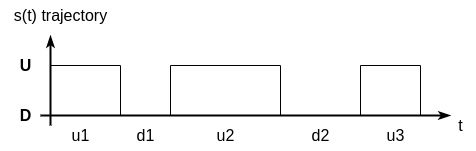
\includegraphics[width=100mm, keepaspectratio]{figures/system_state_partitions.png}
	\caption{ Partitioning the states of the system \cite{DependabilityBMEMIT} }
	\label{fig:system_state_partitions}
\end{figure}

%----------------------------------------------------------------------------
\subsubsection{Mean Values} \label{background-dep-metrics-mean-values}
%----------------------------------------------------------------------------

\paragraph{Mean Time to First Failure} - Mean Time to First Failure -- or MTFF -- denotes the expected time before a given system first encounters a failure that prevents providing correct service. MTFF is calculated with the following formula: \(E\{u_1\}\) and can be visualized using the previously mentioned state partitions as seen in Figure \ref{fig:mtff}.

\begin{figure}[h]
	\centering
	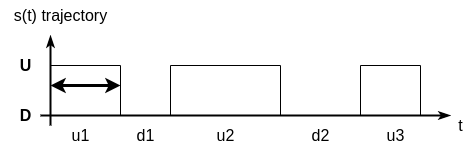
\includegraphics[width=100mm, keepaspectratio]{figures/MTFF.png}
	\caption{ Mean Time to First Failure \cite{DependabilityBMEMIT} }
	\label{fig:mtff}
\end{figure}

\paragraph{Mean Up Time} - Mean Up Time -- or MUT -- is the average duration of time periods during which the system is able to provide correct service. MUT is calculated with the following formula: \(E\{u_i\}\) and can be visualized using the previously mentioned state partitions as seen in Figure \ref{fig:mut}.

\begin{figure}[h]
	\centering
	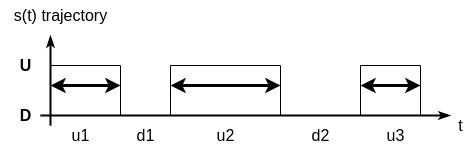
\includegraphics[width=100mm, keepaspectratio]{figures/MUT.png}
	\caption{ Mean Up Time \cite{DependabilityBMEMIT} }
	\label{fig:mut}
\end{figure}

\paragraph{Mean Down Time} - Mean Down Time -- or MDT -- is the average duration of time periods during which the system cannot provide correct service due to failures or maintenance. MDT is calculated with the following formula: \(E\{d_i\}\) and can be visualized using the previously mentioned state partitions as seen in Figure \ref{fig:mdt}.

\begin{figure}[h]
	\centering
	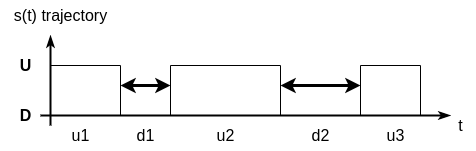
\includegraphics[width=100mm, keepaspectratio]{figures/MDT.png}
	\caption{ Mean Down Time \cite{DependabilityBMEMIT} }
	\label{fig:mdt}
\end{figure}

\paragraph{Mean Time Between Failures} - Mean Time Between Failures -- or MTBF -- denotes the average time between repairable failures of system \cite{KPIMetrics}. MTBF is calculated with the following formula: \(E\{u_i + d_i\} = E\{u_i\} + E\{d_i\}\) (the sum of MUT and MDT) and can be visualized using the previously mentioned state partitions as seen in Figure \ref{fig:mdt}.

\begin{figure}[h]
	\centering
	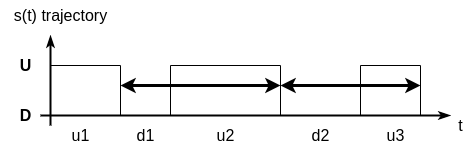
\includegraphics[width=100mm, keepaspectratio]{figures/MTBF.png}
	\caption{ Mean Time Between Failures \cite{DependabilityBMEMIT} }
	\label{fig:mtbf}
\end{figure}

%----------------------------------------------------------------------------
\subsubsection{Probability Functions} \label{background-dep-metrics-prob-funcs}
%----------------------------------------------------------------------------

\paragraph{Availability} - As mentioned earlier in Section \ref{dependability-attributes}, availability describes the probability of correct service in a system. Using the notion of Up and Down system partitions, availability can be calculated with the following formula:

\[
a(t) = P\{ s(t) \in U \}
\]

\paragraph{Reliability} - As mentioned earlier in Section \ref{dependability-attributes}, reliability describes the probability of continuous correct service until the first failure. Using the notion of Up and Down system partitions, availability can be calculated with the following formula:

\[
r(t) = P\{ s(t') \in U, \forall t' < t \}
\]


%----------------------------------------------------------------------------
\section{Kubernetes}
%----------------------------------------------------------------------------

TODO justify containers?

Kubernetes is an open-source platform for managing containerized workloads and services, that facilitates both declarative configuration and automation \cite{KubernetesOverview}. Kubernetes orchestration allows IT professionals to build application services that span multiple containers, schedule those containers across a cluster, scale those containers, and manage the health of those containers over time \cite{KubernetesOverviewRH}.

Kubernetes brings a vast amount of useful features, but a thorough discussion concerning these is out of the scope of this work. However, a brief list is provided below for a clearer context \cite{KubernetesOverview}.

\paragraph{Service discovery and load balancing} - Kubernetes can expose a container using the DNS name or using their own IP address. If traffic to a container is high, Kubernetes is able to load balance and distribute the network traffic so that the deployment is stable \cite{KubernetesOverview}.

\paragraph{Automated rollouts and rollbacks} - Cluster administrators can describe the desired state for the deployed containers using Kubernetes, and it can change the actual state to the desired state at a controlled rate. For example, Kubernetes can automatically create new containers for a deployment, remove existing containers and adopt all their resources to the new container \cite{KubernetesOverview}.

\paragraph{Automatic bin packing} - Kubernetes can automatically schedule the containers of deployments to the nodes in the cluster and aims to achieve the best resource utilization over the whole cluster \cite{KubernetesOverview}.

\paragraph{Self-healing} Kubernetes can automatically restart containers that fail, replace containers, kill containers that do not respond to user-defined health check, and does not advertise them to clients until they are ready to serve \cite{KubernetesOverview}.

%----------------------------------------------------------------------------
\subsection{Cluster Architecture}
%----------------------------------------------------------------------------

TODO
%TODO
diagram from K8s page or own


A Kubernetes cluster consists of a set of worker machines, called nodes, and the control plane. The nodes can be physical or virtual machines depending on the environment and can run anywhere from private data centers to public cloud solutions and even on a single laptop. The control plane manages the worker nodes and the application workload on the cluster \cite{KubernetesArchitecture}.

%----------------------------------------------------------------------------
\subsubsection{Control Plane Components}
%----------------------------------------------------------------------------

The components in the control plane make global decisions about the cluster -- for example scheduling -- and handle cluster events \cite{KubernetesArchitecture}. 

\paragraph{kube-apiserver} The API server exposes the Kubernetes API which acts as the frontend for the Kubernetes control plane. The official Kubernetes command line tool -- \texttt{kubectl} -- and many applications and tools use this API to communicate with the Kubernetes cluster's control plane \cite{KubernetesArchitecture}.

\paragraph{etcd} The etcd is a consistent and highly-available key value storage to keep all Kubernetes cluster data persisted \cite{KubernetesArchitecture}.

\paragraph{kube-scheduler} The kube-scheduler manages the assignment of newly created workloads to nodes based on various factors in order to maintain a balanced cluster state \cite{KubernetesArchitecture}.

\paragraph{kube-controller-manager} This component runs the controller processes in the cluster that watch the shared state of the cluster through the apiserver and make changes attempting to move the current state towards the defined desired state \cite{KubernetesArchitecture}.

\paragraph{cloud-controller-manager} The cloud-controller-manager enables linking the Kubernetes cluster into a cloud provider's API. This permits cloud providers to create a custom integration layer between Kubernetes and their own infrastructure and allows the cloud users to interact with their Kubernetes cluster in a universal way, no matter the underlying cloud infrastructure \cite{KubernetesArchitecture}.

%----------------------------------------------------------------------------
\subsubsection{Node Components}
%----------------------------------------------------------------------------

Node components run on each node in the cluster. Their responsibility is to maintain running the application workloads and to provide the Kubernetes runtime environment \cite{KubernetesArchitecture}.

\paragraph{kubelet} Kubelet is an agent that runs on each node in the cluster, making sure that containers are running in Kubernetes managed resources called Pods (described in section \ref{k8s-pod}).

\paragraph{kube-proxy} This component maintains network rules on each node allowing network communication to application workload running on the cluster from inside or outside of the cluster.

\paragraph{Container Runtime} The container runtime is a software running on each node responsible for managing containers.

%----------------------------------------------------------------------------
\subsection{Common Kubernetes Resources}
%----------------------------------------------------------------------------

The following sections briefly describe some of the commonly used Kubernetes resources in order to enable better comprehension of the thesis work. The resources in Kubernetes can be created inline with \texttt{kubeclt} commands, however the most common way for managing resources is to define them in YAML formatted files and apply them on the cluster.

%----------------------------------------------------------------------------
\subsubsection{Label}
%----------------------------------------------------------------------------

Labels are key-value pairs that are attached to Kubernetes resources. Labels are intended to be used to specify identifying attributes to objects \cite{KubernetesLabel}.

%----------------------------------------------------------------------------
\subsubsection{Namespace}
%----------------------------------------------------------------------------

Namespaces provide a mechanism for isolating groups of resources within a single Kubernetes cluster \cite{KubernetesNamespace}. In case of deploying larger applications, namespaces are a good way of keeping maintenance at a manageable level.

%----------------------------------------------------------------------------
\subsubsection{Pod} \label{k8s-pod}
%----------------------------------------------------------------------------

Pods are the smallest deployable units of computing that can be created and managed in Kubernetes. A Pod is a set of containers, with shared storage and network resources, and a specification for how to run the containers. The containers in a Pod are always co-located, co-scheduled and run in a shared context \cite{KubernetesPod}.

Pods can only be run on nodes. The kube-scheduler automatically assigns every newly created Pods to nodes in the cluster taking into account multiple parameters and constraints. Pods can define scheduling constraints such as so called node selectors which specify the labels a node must have in order to be able to run a Pod \cite{KubernetesNodeSelector}.

%----------------------------------------------------------------------------
\subsubsection{ReplicaSet}
%----------------------------------------------------------------------------

A ReplicaSet's purpose is to maintain a stable set of replica Pods running at any given time. As such, it is often used to guarantee the availability of a specified number of identical Pods \cite{KubernetesReplicaSet}.

%----------------------------------------------------------------------------
\subsubsection{Deployment}
%----------------------------------------------------------------------------

Deployments provide declarative updates for Pods and ReplicaSets based on a declared desired state. Among many things, Deployments can be used to rollout new ReplicaSets, update Pod definitions or scale up and down ReplicaSets to adapt to current workloads \cite{KubernetesDeployment}.

%----------------------------------------------------------------------------
\subsubsection{Service} \label{k8s-service}
%----------------------------------------------------------------------------

A Service is an abstraction layer that defines a logical set of Pods to expose them as a network service inside or outside of the Kubernetes cluster.

Each Pod in the cluster gets its own IP address, however Pods are created and destroyed dynamically to match the current desired state of the cluster. In order to be able to work with durable network addresses that survive Pod lifecycles, Services must be used \cite{KubernetesService}.


%----------------------------------------------------------------------------
\subsubsection{Horizontal Pod Autoscaler}
%----------------------------------------------------------------------------

The Horizontal Pod Autoscaler (HPA) can automatically update a workload resource -- such as a Deployment -- with the aim of automatically scaling the workload to match the current demand. If the load increases and the current number of Pods is not enough to handle it, HPA instructs the workload resource to scale up and to start new Pods. If the load decreases and there are more Pods in a workload than needed to serve requests, HPA tells the workload resource to scale down.

In the background, cluster administrators can configure HPA to watch a specific metric of a workload, e.g. the average CPU utilization or custom defined metric, so the HPA can recognize when the workload resource needs to scale in either direction. For example, when the average CPU utilization breaks from the target boundaries, HPA automatically scales the workload resource to bring back the average CPU utilization into target limits.

%----------------------------------------------------------------------------
\subsubsection{Custom Resource Definition}
%----------------------------------------------------------------------------

Custom Resource Definitions allow cluster administrators to define custom resources as a way to extend the Kubernetes API. Once a custom resources is installed, users can create and access its objects using \texttt{kubectl}, just as they do for built-in resources like Pods. On their own, custom resources enable storing and retrieving structured data. Combined with a custom controller, custom resources provide a true declarative API to implement or adapt arbitrary workflows and use cases in a Kubernetes native way \cite{KubernetesCRD}.

%----------------------------------------------------------------------------
\subsection{Helm} \label{helm}
%----------------------------------------------------------------------------

Helm is a Kubernetes deployment tool for automating creation, packaging, configuration, and deployment of applications and services to Kubernetes clusters \cite{HelmWhatIs}.

Helm works with the concept of Charts which are packages containing all the resource definitions necessary to run an application inside of a Kubernetes cluster. Helm helps mitigating the burden of managing a lot of Kubernetes YAML files with custom configuration values. With Helm, the structural composition of a system and its configuration is separated using template and value files. When a Chart is installed on a cluster, the templates go through the template engine with the provided configuration values resulting in plain Kubernetes resource definitions in YAML format.  This workflow enables Chart users to easily deploy applications tailored to their environment \cite{Helm}.

%----------------------------------------------------------------------------
\section{AWS}
%----------------------------------------------------------------------------

%----------------------------------------------------------------------------
\subsection{CloudFormation} \label{cloudformation}
%----------------------------------------------------------------------------

%----------------------------------------------------------------------------
\subsection{EKS}
%----------------------------------------------------------------------------


%----------------------------------------------------------------------------
\section{Metric collection - Monitoring}
%----------------------------------------------------------------------------

%----------------------------------------------------------------------------
\subsection{Time series}
%----------------------------------------------------------------------------

%----------------------------------------------------------------------------
\subsection{Prometheus}
%----------------------------------------------------------------------------

\begin{itemize}
	\item how it works
	\item the concept of exporters
\end{itemize}

%----------------------------------------------------------------------------
\subsubsection{PromQL} \label{background-promql}
%----------------------------------------------------------------------------

\begin{itemize}
	\item Introduce PromQL
	\item describe query functions that are later used to define dependability metrics
\end{itemize}

%----------------------------------------------------------------------------
\subsubsection{Prometheus Blackbox Exporter}
%----------------------------------------------------------------------------

%----------------------------------------------------------------------------
\subsubsection{Prometheus Adapter}
%----------------------------------------------------------------------------


%----------------------------------------------------------------------------
\subsection{Grafana}
%----------------------------------------------------------------------------


%----------------------------------------------------------------------------
\section{Chaos Engineering}
%----------------------------------------------------------------------------

\begin{itemize}
	\item 
\end{itemize}

%----------------------------------------------------------------------------
\subsection{Chaos Mesh} \label{background-chaos-mesh}
%----------------------------------------------------------------------------

%----------------------------------------------------------------------------
\subsubsection{Chaos Experiments}
%----------------------------------------------------------------------------

%----------------------------------------------------------------------------
\subsubsection{Scheduling Experiments}
%----------------------------------------------------------------------------

%----------------------------------------------------------------------------
\section{Kafka} \label{background-kafka}
%----------------------------------------------------------------------------

\begin{itemize}
	\item overview - pub sub
	\item concepts - Broker, Producer, Consumer, Topic, Partition
\end{itemize}


%----------------------------------------------------------------------------
\chapter{Case study}
%----------------------------------------------------------------------------

\begin{itemize}
	\item Why need a case-study?
	\item Introduce the general problem it solves (naive implementation of Fibonacci)
	\item introduce the general master-job-worker pattern it is based upon

\end{itemize}



%----------------------------------------------------------------------------
\chapter{Design}
%----------------------------------------------------------------------------

%----------------------------------------------------------------------------
\section{Application}
%----------------------------------------------------------------------------

%----------------------------------------------------------------------------
\subsection{Architecture}
%----------------------------------------------------------------------------

architecture diagram

%----------------------------------------------------------------------------
\subsection{Components}
%----------------------------------------------------------------------------

%----------------------------------------------------------------------------
\subsubsection{Backend}
%----------------------------------------------------------------------------

responsibilites + API + health endpoint

%----------------------------------------------------------------------------
\subsubsection{Worker}
%----------------------------------------------------------------------------

responsibilites + API + health endpoint

%----------------------------------------------------------------------------
\subsubsection{Message Queue}
%----------------------------------------------------------------------------

%----------------------------------------------------------------------------
\subsubsection{Database}
%----------------------------------------------------------------------------


%----------------------------------------------------------------------------
\section{Test Framework}
%----------------------------------------------------------------------------


%----------------------------------------------------------------------------
\subsection{Requirements}
%----------------------------------------------------------------------------

\begin{itemize}
	\item Reproducible
	\item Automated
	\item Configurable
	\item Introduce abstract workflow \begin{enumerate}
		\item Prepare infrastructure and application
		\item Generate load
		\item Inject faults
		\item Collect metrics
		\item Store results
	\end{enumerate}
\end{itemize}


%----------------------------------------------------------------------------
\subsection{Load generation}
%----------------------------------------------------------------------------


%----------------------------------------------------------------------------
\subsection{Fault Injection}
%----------------------------------------------------------------------------


%----------------------------------------------------------------------------
\subsubsection{Fault Profiles}
%----------------------------------------------------------------------------

\begin{itemize}
	\item list fault profiles and justification
\end{itemize}

%----------------------------------------------------------------------------
\subsection{Measurement Sequence}
%----------------------------------------------------------------------------

%----------------------------------------------------------------------------
\section{Enhancements}
%----------------------------------------------------------------------------

%----------------------------------------------------------------------------
\subsection{Kafka}
%----------------------------------------------------------------------------

%----------------------------------------------------------------------------
\subsection{Heartbeats}
%----------------------------------------------------------------------------
%----------------------------------------------------------------------------
\chapter{Implementation}
%----------------------------------------------------------------------------

%----------------------------------------------------------------------------
\section{Continuous Delivery}
%----------------------------------------------------------------------------

%----------------------------------------------------------------------------
\section{Framework}
%----------------------------------------------------------------------------

%----------------------------------------------------------------------------
\section{Enhancements}
%----------------------------------------------------------------------------

%----------------------------------------------------------------------------
\subsection{Kafka}
%----------------------------------------------------------------------------

%----------------------------------------------------------------------------
\subsection{Heartbeats}
%----------------------------------------------------------------------------
%----------------------------------------------------------------------------
\chapter{Evaluation}
%----------------------------------------------------------------------------

%----------------------------------------------------------------------------
\section{Continuous Delivery}
%----------------------------------------------------------------------------

%----------------------------------------------------------------------------
\section{Enhancements}
%----------------------------------------------------------------------------

%----------------------------------------------------------------------------
\subsection{Kafka}
%----------------------------------------------------------------------------

%----------------------------------------------------------------------------
\subsection{Heartbeats}
%----------------------------------------------------------------------------

%----------------------------------------------------------------------------
\section{Experiences}
%----------------------------------------------------------------------------

%----------------------------------------------------------------------------
\subsection{Visualizations}
%----------------------------------------------------------------------------

\begin{enumerate}
	\item Grafana dashboards
	\item Jupyter Notebook diagrams
\end{enumerate}
%----------------------------------------------------------------------------
\chapter{Future Work}
%----------------------------------------------------------------------------

\begin{itemize}
	\item database in HA mode (currently single instance)
\end{itemize}
%----------------------------------------------------------------------------
\chapter{Related Works}
%----------------------------------------------------------------------------

The accomplished implementation of the entire thesis work -- including the sample application and the test framework -- realizes a unique set of functionalities in a single system compared to available tools on the market and in the open-source community. However, there are a couple of parts in this system that fulfills a job similar to other existing softwares, like conducting reliability analysis or executing chaos engineering scenarios in Kubernetes based environments. This chapter attempts to collect some of them, without being exhaustive.

%----------------------------------------------------------------------------
\section{Kubernetes Dependability Related Tools}
%----------------------------------------------------------------------------

%----------------------------------------------------------------------------
\subsection{Sonobuoy}
%----------------------------------------------------------------------------

Sonobuoy is diagnostic tool that can analyze and evaluate the state of a running Kubernetes cluster based on various criteria in a non-destructive manner. Among many things, it can be used to perform security of conformance benchmarks and to create inventories collecting all the workloads and operational details on a cluster \cite{Sonobuoy}.

Sonobuoy can be extended to facilitate third-party testing requirements through a plugin system. The plugin that is most related to this thesis work is the Reliability Scanner plugin \cite{SonobuoyReliabilityScanner}. The Reliability Scanner captures and inspects good practices for operating workloads reliably on Kubernetes which includes the existence verification of  probes, ownership indicators and Quality of Service configurations.

Compared to the implemented testing framework described in previous sections this tool carries the following advantages and disadvantages (without being exhaustive):

\paragraph{Pros} Sonobuoy Reliability Scanner plugin is a great tool to check general configurations that can cause severe anomalies if not set correctly. The results are collected into well organized reports which are easy to comprehend for all stakeholders.

\paragraph{Cons} The Sonobuoy Reliability Scanner is only able to verify the static features of the system -- the configuration. It cannot be used to check the actual functional reliability of a system which can dynamically change over time. It may easily happen, that the inspected configurations are all in place, but the system is still not able to operate in a reliable manner.

%----------------------------------------------------------------------------
\section{Chaos Engineering Tools}
%----------------------------------------------------------------------------

%----------------------------------------------------------------------------
\subsection{Gremlin}
%----------------------------------------------------------------------------

Gremlin is a comprehensive, enterprise ready Chaos Engineering platform to enable its users to proactively improve their systems' reliability \cite{Gremlin}. It is provided with a SaaS model, where customers can easily access and manage their chaos experiments and scenarios through a browser based interface. Users only have to install Gremlin agents to their machines and connect them to their Gremlin account.

Gremlin is able to inject many kinds of failures into a system. These can impact resources, network traffic or the processes running on the infrastructure. Similarly to Chaos Mesh, Gremlin can also schedule chaos experiments and summarize the attack reports in an organized way.

Compared to the implemented testing framework described in previous sections this tool carries the following advantages and disadvantages (without being exhaustive):

\paragraph{Pros} Gremlin offers a full fledged platform with a well organized graphical interface that can get users started quickly. It is able to perform chaos engineering experiments in many kind of infrastructural environments -- not only on Kubernetes -- independent from cloud providers.

\paragraph{Cons} Gremlin also supports performing custom checks during a failure scenario execution, however, the results of these status checks are only binary. It is not easily achievable to define and track complex dependability metrics while conducting chaos experiments.

%----------------------------------------------------------------------------
\subsection{Litmus}
%----------------------------------------------------------------------------

Litmus is an open-source cross-cloud Chaos Engineering framework that lets developers and site reliability engineers to define complex set of chaos experiments with various kinds of status checks to form workflows that can identify weaknesses in a Kubernetes based system \cite{Litmus}.

Similarly to Chaos Mesh, Litmus can also be used with the help of Kubernetes Custom Resource Definitions to install the necessary components of Litmus that control and execute the fault injections.

Compared to the implemented testing framework described in previous sections this tool carries the following advantages and disadvantages (without being exhaustive):

\paragraph{Pros} Litmus can be seamlessly integrated into existing CI pipelines without modifying them. Users can configure Litmus to continuously watch target resources on a Kubernetes cluster (\eg Deployments) and trigger chaos experiments whenever these targets change. This feature allows conducting extensive chaos experiments in an automated way which can prove to be quite useful for example in staging environments before releasing an application into production.

\paragraph{Cons} Similarly as Gremlin, it is not possible with Litmus to combine more complex metrics and dynamic properties with the chaos experiment execution to assess system characteristics more thoroughly.

%----------------------------------------------------------------------------
\chapter{Summary}
%----------------------------------------------------------------------------

The ever transforming market and the conceptual changes of software delivery drive companies to swiftly move their IT infrastructure and services into the cloud. Cloud computing offers countless advantages both for enterprises and their customers, however, adopting cloud solutions the right way is not an easy task. There are many pitfalls concerning application architecture, implementation, deployment and maintenance that can be easily overseen even by experienced system developers. As more and more critical applications are migrated into the cloud, companies have to be sure, that their systems are able to function reliably to avoid severe losses in case of unexpected failures. This demands the existence of various tools that can consequently check the dependability of highly distributed and dynamic applications and reveal their weaknesses.

This thesis work first introduced Kubernetes, the widely popular open-source platform for containerized workload orchestration in the cloud, describing its main features and concepts used throughout this project.

Following that, the design and implementation of a sample application were presented which was later used during the dependability analyses. The sample application is a small, Kubernetes based distributed system, composed of both stateful and stateless components that support scalability. It conforms to the most important microservice requirements like containerization, separation of responsibilities and observability.

Afterwards, the document expressed the need for a configurable, automated test framework that can be used for measuring the dependability of Kubernetes based applications. The related chapter described the design process and implementation of such a tool in detail, highlighting its capabilities like automatic load generation, fault injection and monitoring. With the help of this framework, baseline measurements were conducted against the sample application to assess its dependability characteristics in its original form. The initial measurement results were analyzed and served as good basis to design further improvements on the sample application to achieve a more robust system.

With the sample application and the baseline results being ready, enhancements could be implemented to harden the dependability of the system. The next parts of the thesis explored the possible architectural layers, where additional development could take place. Later on, two specific improvements were carried out, a custom implementation and the integration of Kafka into the sample application. The effects of these two enhancements on the sample application's dependability were measured with the formerly created test framework and conclusions were drawn based on the results. The key takeaways were that it is worth to spend time with making improvements on the application level before integrating complex third-party systems, but when adapting these softwares, one has to make sure not to introduce additional weaknesses into the system with incomplete configurations.

The document continues with a discussion about the possible directions of future developments. These include the improvements on the test framework and the extension of possible enhancement options.

Finally, the thesis ends with a brief discussion about the related works. Although the presented project carries a unique set of functionalities, there are existing tools and software components that realize similar use-cases as the parts of the implemented system, like reliability analysis and chaos engineering.

%%----------------------------------------------------------------------------
\chapter{\LaTeX-eszközök}
\label{sec:LatexTools}
%----------------------------------------------------------------------------
\section{A szerkesztéshez használatos eszközök}
%----------------------------------------------------------------------------
Ez a sablon TeXstudio 2.8.8 szerkesztővel készült. A TeXstudio egy platformfüggetlen, Windows, Linux és Mac OS alatt is elérhető \LaTeX-szerkesztőprogram számtalan hasznos szolgáltatással (\refstruc{fig:TeXstudio}). A szoftver ingyenesen letölthető\footnote{A TeXstudio hivatalos oldala: \url{http://texstudio.sourceforge.net/}}.

\begin{figure}[!ht]
\centering
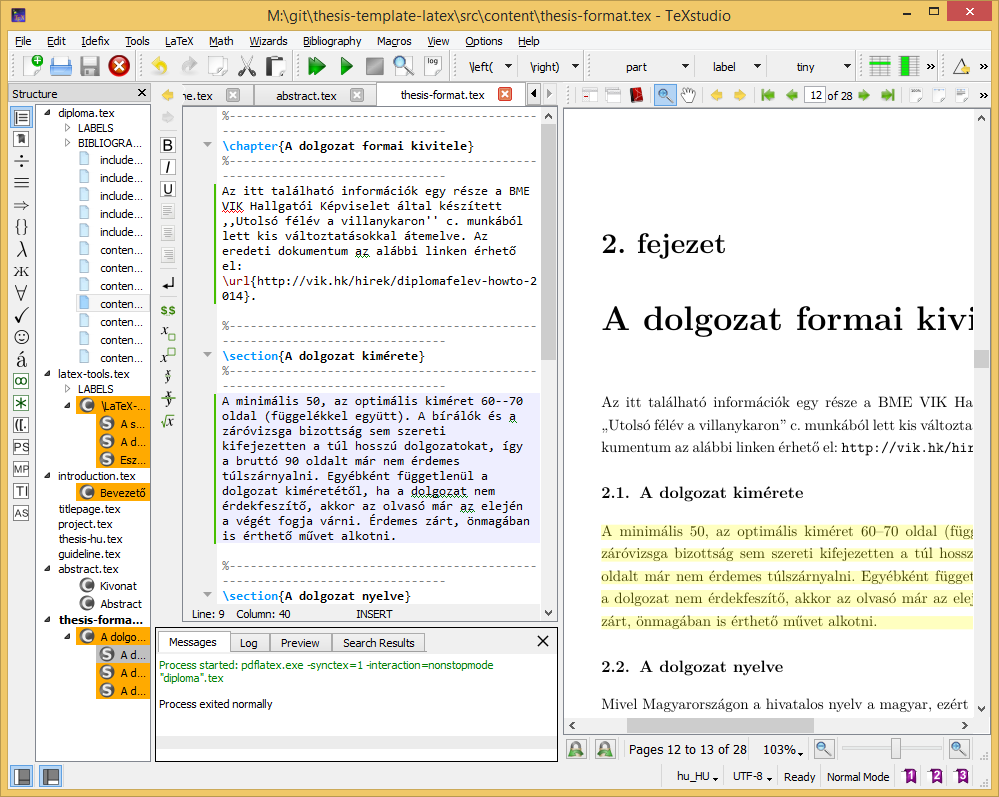
\includegraphics[width=150mm, keepaspectratio]{figures/TeXstudio.png}
\caption{A TeXstudio \LaTeX-szerkesztő.}
\label{fig:TeXstudio}
\end{figure}

A TeXstudio telepítése után érdemes még letölteni a magyar nyelvű helyesírásellenőrző-szótárakat hozzá. A TeXstudio az OpenOffice-hoz használatos formátumot tudja kezelni. A TeXstudio beállításainál a \verb+General+ fülön a \verb+Dictionaries+ résznél tudjuk megadni, hogy melyik szótárat használja.

Egy másik használható Windows alapú szerkesztőprogram a LEd\footnote{A LEd hivatalos oldala: \url{http://www.latexeditor.org/}} (LaTeX Editor), a TeXstudio azonban stabilabb, gyorsabb, és jobban használható.

%----------------------------------------------------------------------------
\section{A dokumentum lefordítása Windows alatt}
%----------------------------------------------------------------------------
A TeXstudio és a LEd kizárólag szerkesztőprogram (bár az utóbbiban DVI-nézegető is van), így a dokumentum fordításához szükséges eszközöket nem tartalmazza. Windows alatt alapvetően két lehetőség közül érdemes választani: MiKTeX (\url{http://miktex.org/}) és TeX Live (\url{http://www.tug.org/texlive/}) programcsomag. Az utóbbi működik Mac OS X, GNU/Linux alatt és Unix-származékokon is. A MiKTeX egy alapcsomag telepítése után mindig letölti a használt funkciókhoz szükséges, de lokálisan hiányzó \TeX-csomagokat, míg a TeX Live DVD ISO verzóban férhető hozzá. Ez a dokumentum TeX Live 2008 programcsomag segítségével fordult, amelynek DVD ISO verziója a megadott oldalról letölthető. A sablon lefordításához a disztribúcióban szereplő \verb+magyar.ldf+ fájlt a \verb+http://www.math.bme.hu/latex/+ változatra kell cserélni, vagy az utóbbi változatot be kell másolni a projekt-könyvtárba (ahogy ezt meg is tettük a sablonban) különben anomáliák tapasztalhatók a dokumentumban (pl. az ábra- és táblázat-aláírások formátuma nem a beállított lesz, vagy bizonyos oldalakon megjelenik alapértelmezésben egy fejléc). A TeX Live 2008-at még nem kell külön telepíteni a gépre, elegendő DVD-ről (vagy az ISO fájlból közvetlenül, pl. DaemonTools-szal) használni.

Ha a MiKTeX csomagot használjuk, akkor parancssorból a következő módon tudjuk újrafordítani a teljes dokumentumot:

\begin{lstlisting}[language=bash,frame=single,float=!ht]
$ texify -p thesis.tex
\end{lstlisting}

A \verb+texify+ parancs a MiKTex programcsomag \verb+miktex/bin+ alkönyvtárában található. A parancs gondoskodik arról, hogy a szükséges lépéseket (fordítás, hivatkozások generálása stb.) a megfelelő sorrendben elvégezze. A \verb+-p+ kapcsoló hatására PDF-et generál. A fordítást és az ideiglenes fájlok törlését elvégezhetjük a sablonhoz mellékelt \verb+manual_build.bat+ szkript segítségével is.

A \TeX-eszközöket tartalmazó programcsomag binárisainak elérési útját gyakran be kell állítani a szerkesztőprogramban, például TeXstudio esetén legegyszerűbben az \verb+Options / Configure TeXstudio... / Commands+ menüponttal előhívott dialógusablakban tehetjük ezt meg.

A PDF-\LaTeX~használata esetén a generált dokumentum közvetlenül PDF-formátumban áll rendelkezésre. Amennyiben a PDF-fájl egy PDF-nézőben (pl. Adobe Acrobat Reader vagy Foxit PDF Reader) meg van nyitva, akkor a fájlleírót a PDF-néző program tipikusan lefoglalja. Ilyen esetben a dokumentum újrafordítása hibaüzenettel kilép. Ha bezárjuk és újra megnyitjuk a PDF dokumentumot, akkor pedig a PDF-nézők többsége az első oldalon nyitja meg a dokumentumot, nem a legutóbb olvasott oldalon. Ezzel szemben például az egyszerű és ingyenes \textcolor{blue}{Sumatra PDF} nevű program képes arra, hogy a megnyitott dokumentum megváltozását detektálja, és frissítse a nézetet az aktuális oldal megtartásával.

%----------------------------------------------------------------------------
\section{Eszközök Linuxhoz}
%----------------------------------------------------------------------------
Linux operációs rendszer alatt is rengeteg szerkesztőprogram van, pl. a KDE alapú Kile jól használható. Ez ingyenesen letölthető, vagy éppenséggel az adott Linux-disztribúció eleve tartalmazza, ahogyan a dokumentum fordításához szükséges csomagokat is. Az Ubuntu Linux disztribúciók alatt például legtöbbször a \verb+texlive-*+ csomagok telepítésével használhatók a \LaTeX-eszközök. A jelen sablon fordításához szükséges csomagok (kb. 0,5 GB) az alábbi paranccsal telepíthetők:

\begin{lstlisting}[language=bash,morekeywords={sudo,apt\-get},alsoletter={-},breaklines=true]
$ sudo apt-get install texlive-latex-extra texlive-fonts-extra texlive-fonts-recommended texlive-xetex texlive-science
\end{lstlisting}

Amennyiben egy újabb csomag hozzáadása után hiányzó fájlra utaló hibát kapunk a fordítótól, telepítenünk kell az azt tartalmazó TeX Live csomagot. Ha pl. a \verb+bibentry+ csomagot szeretnénk használni, futtassuk az alábbi parancsot:

\begin{lstlisting}[language=bash,morekeywords={apt\-cache},alsoletter={-},breaklines=true]
$ apt-cache search bibentry
texlive-luatex - TeX Live: LuaTeX packages
\end{lstlisting}

Majd telepítsük fel a megfelelő TeX Live csomagot, jelen esetben a `texlive-lualatex`-et. (Egy LaTeX csomag több TeX Live csomagban is szerepelhet.)

Ha gyakran szerkesztünk más \LaTeX dokumentumokat is, kényelmes és biztos megoldás a teljes TeX Live disztribúció telepítése, ez azonban kb. 4 GB helyet igényel.

\begin{lstlisting}[language=bash,morekeywords={sudo,apt\-get},alsoletter={-},breaklines=true]
sudo apt-get install texlive-full
\end{lstlisting}

%%----------------------------------------------------------------------------
\chapter{A dolgozat formai kivitele}
%----------------------------------------------------------------------------
Az itt található információk egy része a BME VIK Hallgatói Képviselet által készített ,,Utolsó félév a villanykaron'' c. munkából lett kis változtatásokkal átemelve. Az eredeti dokumentum az alábbi linken érhető el: \url{http://vik.hk/hirek/diplomafelev-howto-2015}.

%----------------------------------------------------------------------------
\section{A dolgozat kimérete}
%----------------------------------------------------------------------------
Szakdolgozat esetében minimum 30, 45 körüli ajánlott oldalszám lehet az iránymutató. De mindenképp érdemes rákérdezni a konzulensnél is az elvárásokra, mert tanszékenként változóak lehetnek az elvárások.

Mesterképzésen a Diplomatervezés 1 esetében a beszámoló még inkább az Önálló laboratóriumi beszámolókhoz hasonlít, tanszékenként eltérő formai követelményekkel, -- egy legalább 30 oldal körüli dolgozat az elvárt -- és az elmúlt fél éves munkáról szól. De egyben célszerű, ha ez a végleges diplomaterv alapja is. (A végleges 60-90 oldal körülbelül a hasznos részre nézve)


%----------------------------------------------------------------------------
\section{A dolgozat nyelve}
%----------------------------------------------------------------------------
Mivel Magyarországon a hivatalos nyelv a magyar, ezért alapértelmezésben magyarul kell megírni a dolgozatot. Aki külföldi posztgraduális képzésben akar részt venni, nemzetközi szintű tudományos kutatást szeretne végezni, vagy multinacionális cégnél akar elhelyezkedni, annak célszerű angolul megírnia diplomadolgozatát. Mielőtt a hallgató az angol nyelvű verzió mellett dönt, erősen ajánlott mérlegelni, hogy ez mennyi többletmunkát fog a hallgatónak jelenteni fogalmazás és nyelvhelyesség terén, valamint -- nem utolsó sorban -- hogy ez mennyi többletmunkát fog jelenteni a konzulens illetve bíráló számára. Egy nehezen olvasható, netalán érthetetlen szöveg teher minden játékos számára.

%----------------------------------------------------------------------------
\section{A dokumentum nyomdatechnikai kivitele}
%----------------------------------------------------------------------------
A dolgozatot A4-es fehér lapra nyomtatva, 2,5 centiméteres margóval (+1~cm kötésbeni), 11--12 pontos betűmérettel, talpas betűtípussal és másfeles sorközzel célszerű elkészíteni.

Annak érdekében, hogy a dolgozat külsőleg is igényes munka benyomását keltse, érdemes figyelni az alapvető tipográfiai szabályok betartására~\cite{Jeney}.

%% !TeX spellcheck = hu_HU
% !TeX encoding = UTF-8
% !TeX program = xelatex
%----------------------------------------------------------------------------
\chapter{A \LaTeX-sablon használata}
%----------------------------------------------------------------------------

Ebben a fejezetben röviden, implicit módon bemutatjuk a sablon használatának módját, ami azt jelenti, hogy sablon használata ennek a dokumentumnak a forráskódját tanulmányozva válik teljesen világossá. Amennyiben a szoftver-keretrendszer telepítve van, a sablon alkalmazása és a dolgozat szerkesztése \LaTeX-ben a sablon segítségével tapasztalataink szerint jóval hatékonyabb, mint egy WYSWYG (\emph{What You See is What You Get}) típusú szövegszerkesztő esetén (pl. Microsoft Word, OpenOffice).

%----------------------------------------------------------------------------
\section{Címkék és hivatkozások}
%----------------------------------------------------------------------------
A \LaTeX~dokumentumban címkéket (\verb+\label+) rendelhetünk ábrákhoz, táblázatokhoz, fejezetekhez, listákhoz, képletekhez stb. Ezekre a dokumentum bármely részében hivatkozhatunk, a hivatkozások automatikusan feloldásra kerülnek.

A sablonban makrókat definiáltunk a hivatkozások megkönnyítéséhez. Ennek megfelelően minden ábra (\emph{figure}) címkéje \verb+fig:+ kulcsszóval kezdődik, míg minden táblázat (\emph{table}), képlet (\emph{equation}), fejezet (\emph{section}) és lista (\emph{listing}) rendre a \verb+tab:+, \verb+eq:+, \verb+sec:+ és \verb+lst:+ kulcsszóval kezdődik, és a kulcsszavak után tetszőlegesen választott címke használható. Ha ezt a konvenciót betartjuk, akkor az előbbi objektumok számára rendre a \verb+\figref+, \verb+\tabref+, \verb+\eqref+, \verb+\sectref+ és \verb+\listref+ makrókkal hivatkozhatunk. A makrók paramétere a címke, amelyre hivatkozunk (a kulcsszó nélkül). Az összes említett hivatkozástípus, beleértve az \verb+\url+ kulcsszóval bevezetett web-hivatkozásokat is a  \verb+hyperref+\footnote{Segítségével a dokumentumban megjelenő hivatkozások nem csak dinamikussá válnak, de színezhetők is, bővebbet erről a csomag dokumentációjában találunk. Ez egyúttal egy példa lábjegyzet írására.} csomagnak köszönhetően aktívak a legtöbb PDF-nézegetőben, rájuk kattintva a dokumentum megfelelő oldalára ugrik a PDF-néző vagy a megfelelő linket megnyitja az alapértelmezett böngészővel. A \verb+hyperref+ csomag a kimeneti PDF-dokumentumba könyvjelzőket is készít a tartalomjegyzékből. Ez egy szintén aktív tartalomjegyzék, amelynek elemeire kattintva a nézegető behozza a kiválasztott fejezetet.

%----------------------------------------------------------------------------
\section{Ábrák és táblázatok}
%----------------------------------------------------------------------------
Használjunk vektorgrafikus ábrákat, ha van rá módunk. PDFLaTeX használata esetén PDF formátumú ábrákat lehet beilleszteni könnyen, az EPS (PostScript) vektorgrafikus képformátum beillesztését a PDFLaTeX közvetlenül nem támogatja (de lehet konvertálni, lásd később). Ha vektorgrafikus formában nem áll rendelkezésünkre az ábra, akkor a  veszteségmentes PNG, valamint a veszteséges JPEG formátumban érdemes elmenteni.  Figyeljünk arra, hogy ilyenkor a képek felbontása elég nagy legyen ahhoz, hogy nyomtatásban is megfelelő minőséget nyújtson (legalább 300 dpi javasolt). A dokumentumban felhasznált képfájlokat a dokumentum forrása mellett érdemes tartani, archiválni, mivel ezek hiányában a dokumentum nem fordul újra. Ha lehet, a vektorgrafikus képeket vektorgrafikus formátumban is érdemes elmenteni az újrafelhasználhatóság (az átszerkeszthetőség) érdekében.

Kapcsolási rajzok legtöbbször kimásolhatók egy vektorgrafikus programba (pl. CorelDraw) és onnan nagyobb felbontással raszterizálva kimenthatők PNG formátumban. Ugyanakkor kiváló ábrák készíthetők Microsoft Visio vagy hasonló program használatával is: Visio-ból az ábrák közvetlenül PDF-be is menthetők.

Lehetőségeink Matlab ábrák esetén:
\begin{itemize}
	\item Képernyőlopás (\emph{screenshot}) is elfogadható minőségű lehet a dokumentumban, de általában jobb felbontást is el lehet érni más módszerrel.
	\item A Matlab ábrát a \verb+File/Save As+ opcióval lementhetjük PNG formátumban (ugyanaz itt is érvényes, mint korábban, ezért nem javasoljuk).
	\item A Matlab ábrát az \verb+Edit/Copy figure+ opcióval kimásolhatjuk egy vektorgrafikus programba is és onnan nagyobb felbontással raszterizálva kimenthatjük PNG formátumban (nem javasolt).
	\item Javasolt megoldás: az ábrát a \verb+File/Save As+ opcióval EPS \emph{vektorgrafikus} formátumban elmentjük, PDF-be konvertálva beillesztjük a dolgozatba.
\end{itemize}
Az EPS kép az \verb+epstopdf+ programmal\footnote{a korábban említett \LaTeX-disztribúciókban megtalálható} konvertálható PDF formátumba. Célszerű egy batch-fájlt készíteni az összes EPS ábra lefordítására az alábbi módon (ez Windows alatt működik).
\begin{lstlisting}[language=]
@echo off
for %%j in (*.eps) do (
  echo converting file "%%j"
  epstopdf "%%j"
)
echo done .
\end{lstlisting}

Egy ilyen parancsfájlt (\verb+convert.cmd+) elhelyeztük a sablon \verb+figures\eps+ könyvtárába, így a felhasználónak csak annyi a dolga, hogy a \verb+figures\eps+ könyvtárba kimenti az EPS formátumú vektorgrafikus képet, majd lefuttatja a \verb+convert.cmd+ parancsfájlt, ami PDF-be konvertálja az EPS fájlt.

Ezek után a PDF-ábrát ugyanúgy lehet a dokumentumba beilleszteni, mint a PNG-t vagy a JPEG-et. A megoldás előnye, hogy a lefordított dokumentumban is vektorgrafikusan tárolódik az ábra, így a mérete jóval kisebb, mintha raszterizáltuk volna beillesztés előtt. Ez a módszer minden -- az EPS formátumot ismerő -- vektorgrafikus program (pl. CorelDraw) esetén is használható.

A képek beillesztésére \az+\refstruc{sec:LatexTools}ben mutattunk be példát (\refstruc{fig:TeXstudio}). Az előző mondatban egyúttal az automatikusan feloldódó ábrahivatkozásra is láthatunk példát. Több képfájlt is beilleszthetünk egyetlen ábrába. Az egyes képek közötti horizontális és vertikális margót metrikusan szabályozhatjuk (\refstruc{fig:HVSpaces}). Az ábrák elhelyezését számtalan tipográfiai szabály egyidejű teljesítésével a fordító maga végzi, a dokumentum írója csak preferenciáit jelezheti a fordító felé (olykor ez bosszúságot is okozhat, ilyenkor pl. a kép méretével lehet játszani).

\begin{figure}[!ht]
	\centering
	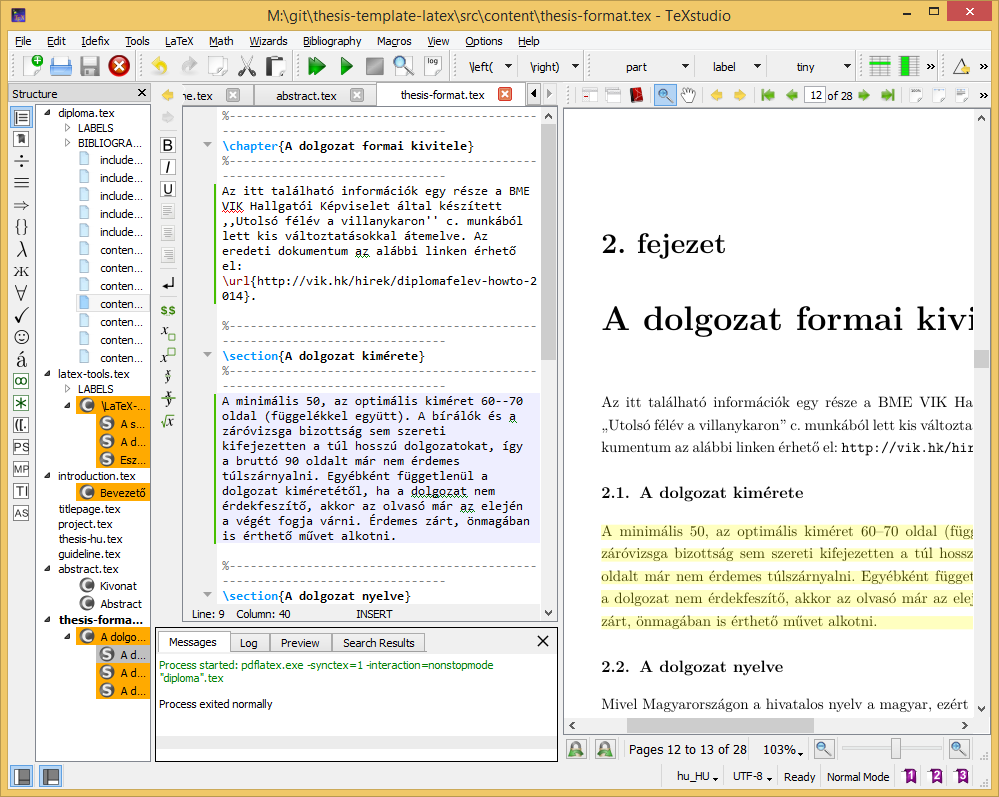
\includegraphics[width=67mm, keepaspectratio]{figures/TeXstudio.png}\hspace{1cm}
	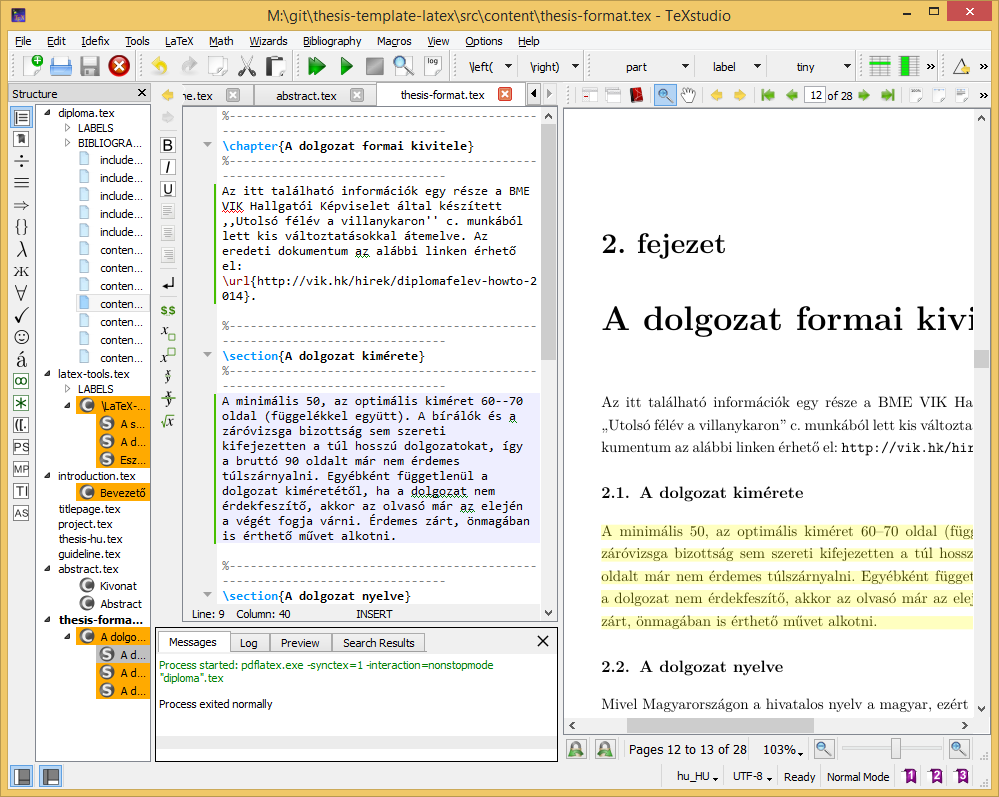
\includegraphics[width=67mm, keepaspectratio]{figures/TeXstudio.png}\\\vspace{5mm}
	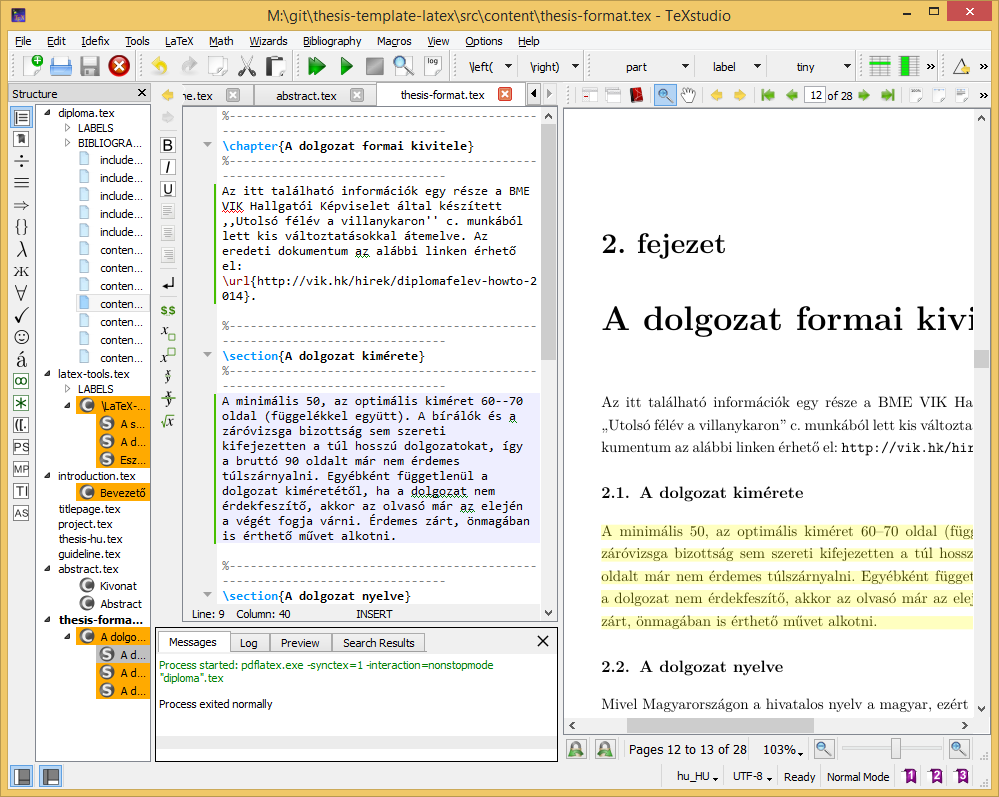
\includegraphics[width=67mm, keepaspectratio]{figures/TeXstudio.png}\hspace{1cm}
	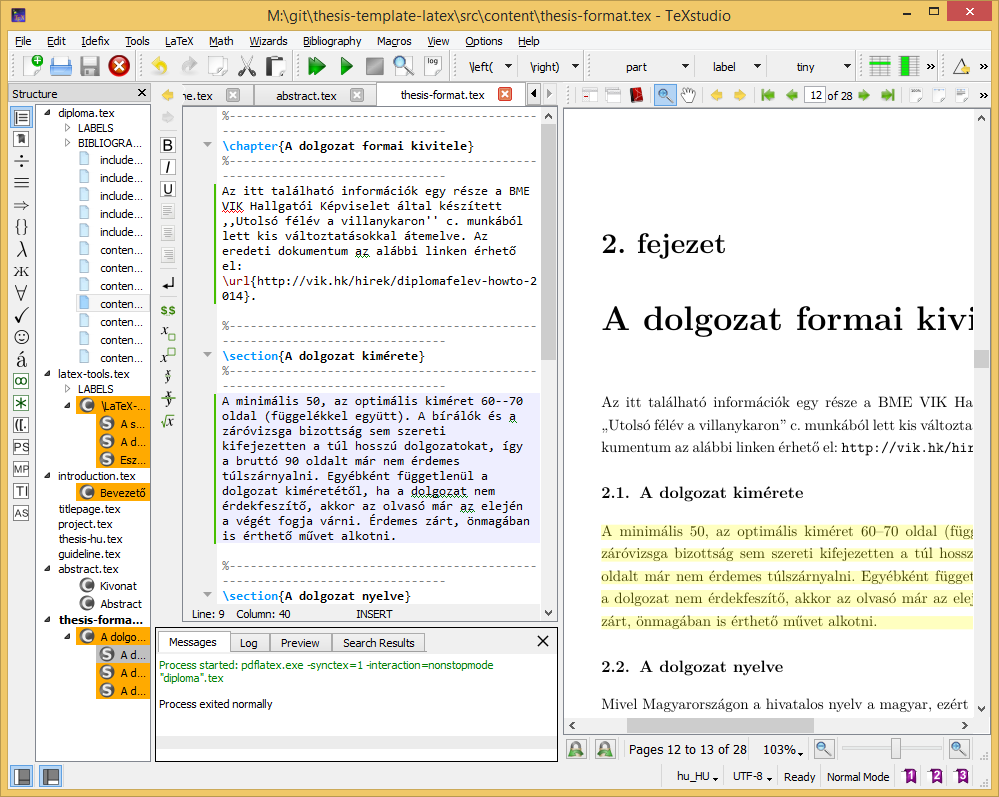
\includegraphics[width=67mm, keepaspectratio]{figures/TeXstudio.png}
	\caption{Több képfájl beillesztése esetén térközöket is érdemes használni.}
	\label{fig:HVSpaces}
\end{figure}

A táblázatok használatára \aref{tab:TabularExample}~táblázat mutat példát. A táblázatok formázásához hasznos tanácsokat találunk a \verb+booktabs+ csomag dokumentációjában.

\begin{table}[ht]
	\footnotesize
	\centering
	\begin{tabular}{ l c c }
		\toprule
		Órajel & Frekvencia & Cél pin \\
		\midrule
		CLKA & 100 MHz & FPGA CLK0\\
		CLKB & 48 MHz  & FPGA CLK1\\
		CLKC & 20 MHz  & Processzor\\
		CLKD & 25 MHz  & Ethernet chip \\
		CLKE & 72 MHz  & FPGA CLK2\\
		XBUF & 20 MHz  & FPGA CLK3\\
		\bottomrule
	\end{tabular}
	\caption{Az órajel-generátor chip órajel-kimenetei.}
	\label{tab:TabularExample}
\end{table}


%----------------------------------------------------------------------------
\section{Felsorolások és listák}
%----------------------------------------------------------------------------
Számozatlan felsorolásra mutat példát a jelenlegi bekezdés:
\begin{itemize}
	\item \emph{első bajusz:} ide lehetne írni az első elem kifejését,
	\item \emph{második bajusz:} ide lehetne írni a második elem kifejését,
	\item \emph{ez meg egy szakáll:} ide lehetne írni a harmadik elem kifejését.
\end{itemize}

Számozott felsorolást is készíthetünk az alábbi módon:
\begin{enumerate}
	\item \emph{első bajusz:} ide lehetne írni az első elem kifejését, és ez a kifejtés így néz ki, ha több sorosra sikeredik,
	\item \emph{második bajusz:} ide lehetne írni a második elem kifejését,
	\item \emph{ez meg egy szakáll:} ide lehetne írni a harmadik elem kifejését.
\end{enumerate}
A felsorolásokban sorok végén vessző, az utolsó sor végén pedig pont a szokásos írásjel. Ez alól kivételt képezhet, ha az egyes elemek több teljes mondatot tartalmaznak.

Listákban a dolgozat szövegétől elkülönítendő kódrészleteket, programsorokat, pszeudo-kódokat jeleníthetünk meg (\ref{lst:Example}.~kódrészlet).
\begin{lstlisting}[language=tex,caption=A fenti számozott felsorolás \LaTeX-forráskódja,label=lst:Example]
\begin{enumerate}
	\item \emph{els(*@ő@*) bajusz:} ide lehetne írni az els(*@ő@*) elem kifejését,
	és ez a kifejtés így néz ki, ha több sorosra sikeredik,
	\item \emph{második bajusz:} ide lehetne írni a második elem kifejését,
	\item \emph{ez meg egy szakáll:} ide lehetne írni a harmadik elem kifejését.
\end{enumerate}
\end{lstlisting}
A lista keretét, háttérszínét, egész stílusát megválaszthatjuk. Ráadásul különféle programnyelveket és a nyelveken belül kulcsszavakat is definiálhatunk, ha szükséges. Erről bővebbet a \verb+listings+ csomag hivatalos leírásában találhatunk.

%----------------------------------------------------------------------------
\section{Képletek}
%----------------------------------------------------------------------------
Ha egy formula nem túlságosan hosszú, és nem akarjuk hivatkozni a szövegből, mint például a $e^{i\pi}+1=0$ képlet, \emph{szövegközi képletként} szokás leírni. Csak, hogy másik példát is lássunk, az $U_i=-d\Phi/dt$ Faraday-törvény a $\rot E=-\frac{dB}{dt}$ differenciális alakban adott Maxwell-egyenlet felületre vett integráljából vezethető le. Látható, hogy a \LaTeX-fordító a sorközöket betartja, így a szöveg szedése esztétikus marad szövegközi képletek használata esetén is.

Képletek esetén az általános konvenció, hogy a kisbetűk skalárt, a kis félkövér betűk ($\mathbf{v}$) oszlopvektort -- és ennek megfelelően $\mathbf{v}^T$ sorvektort -- a kapitális félkövér betűk ($\mathbf{V}$) mátrixot jelölnek. Ha ettől el szeretnénk térni, akkor az alkalmazni kívánt jelölésmódot célszerű külön alfejezetben definiálni. Ennek megfelelően, amennyiben $\mathbf{y}$ jelöli a mérések vektorát, $\mathbf{\vartheta}$ a paraméterek vektorát és $\hat{\mathbf{y}}=\mathbf{X}\vartheta$ a paraméterekben lineáris modellt, akkor a \emph{Least-Squares} értelemben optimális paraméterbecslő $\hat{\mathbf{\vartheta}}_{LS}=(\mathbf{X}^T\mathbf{X})^{-1}\mathbf{X}^T\mathbf{y}$ lesz.

Emellett kiemelt, sorszámozott képleteket is megadhatunk, ennél az \verb+equation+ és a \verb+eqnarray+ környezetek helyett a korszerűbb \verb+align+ környezet alkalmazását javasoljuk (több okból, különféle problémák elkerülése végett, amelyekre most nem térünk ki). Tehát
\begin{align}
\dot{\mathbf{x}}&=\mathbf{A}\mathbf{x}+\mathbf{B}\mathbf{u},\\
\mathbf{y}&=\mathbf{C}\mathbf{x},
\end{align}
ahol $\mathbf{x}$ az állapotvektor, $\mathbf{y}$ a mérések vektora és $\mathbf{A}$, $\mathbf{B}$ és $\mathbf{C}$ a rendszert leíró paramétermátrixok. Figyeljük meg, hogy a két egyenletben az egyenlőségjelek egymáshoz igazítva jelennek meg, mivel a mindkettőt az \& karakter előzi meg a kódban. Lehetőség van számozatlan kiemelt képlet használatára is, például
\begin{align}
\dot{\mathbf{x}}&=\mathbf{A}\mathbf{x}+\mathbf{B}\mathbf{u},\nonumber\\
\mathbf{y}&=\mathbf{C}\mathbf{x}\nonumber.
\end{align}
Mátrixok felírására az $\mathbf{A}\mathbf{x}=\mathbf{b}$ inhomogén lineáris egyenlet részletes kifejtésével mutatunk példát:
\begin{align}
\begin{bmatrix}
a_{11} & a_{12} & \dots & a_{1n}\\
a_{21} & a_{22} & \dots & a_{2n}\\
\vdots & \vdots & \ddots & \vdots\\
a_{m1} & a_{m2} & \dots & a_{mn}
\end{bmatrix}
\begin{pmatrix}x_1\\x_2\\\vdots\\x_n\end{pmatrix}=
\begin{pmatrix}b_1\\b_2\\\vdots\\b_m\end{pmatrix}.
\end{align}
A \verb+\frac+ utasítás hatékonyságát egy általános másodfokú tag átviteli függvényén keresztül mutatjuk be, azaz
\begin{align}
W(s)=\frac{A}{1+2T\xi s+s^2T^2}.
\end{align}
A matematikai mód minden szimbólumának és képességének a bemutatására természetesen itt nincs lehetőség, de gyors referenciaként hatékonyan használhatók a következő linkek:\\
\indent\url{http://www.artofproblemsolving.com/LaTeX/AoPS_L_GuideSym.php},\\
\indent\url{http://www.ctan.org/tex-archive/info/symbols/comprehensive/symbols-a4.pdf},\\
\indent\url{ftp://ftp.ams.org/pub/tex/doc/amsmath/short-math-guide.pdf}.\\
Ez pedig itt egy magyarázat, hogy miért érdemes \verb+align+ környezetet használni:\\
\indent\url{http://texblog.net/latex-archive/maths/eqnarray-align-environment/}.

%----------------------------------------------------------------------------
\section{Irodalmi hivatkozások}
\label{sec:HowtoReference}
%----------------------------------------------------------------------------
Egy \LaTeX~dokumentumban az irodalmi hivatkozások definíciójának két módja van. Az egyik a \verb+\thebibliograhy+ környezet használata a dokumentum végén, az \verb+\end{document}+ lezárás előtt.
\begin{lstlisting}[language=tex]
\begin{thebibliography}{9}

\bibitem{Lamport94} Leslie Lamport, \emph{\LaTeX: A Document Preparation System}.
Addison Wesley, Massachusetts, 2nd Edition, 1994.

\end{thebibliography}
\end{lstlisting}

Ezek után a dokumentumban a \verb+\cite{Lamport94}+ utasítással hivatkozhatunk a forrásra. A fenti megadás viszonylag kötetlen, a szerző maga formázza az irodalomjegyzéket (ami gyakran inkonzisztens eredményhez vezet).

Egy sokkal professzionálisabb módszer a BiB\TeX{} használata, ezért ez a sablon is ezt támogatja. Ebben az esetben egy külön szöveges adatbázisban definiáljuk a forrásmunkákat, és egy külön stílusfájl határozza meg az irodalomjegyzék kinézetét. Ez, összhangban azzal, hogy külön formátumkonvenció határozza meg a folyóirat-, a könyv-, a konferenciacikk- stb. hivatkozások kinézetét az irodalomjegyzékben (a sablon használata esetén ezzel nem is kell foglalkoznia a hallgatónak, de az eredményt célszerű ellenőrizni). felhasznált hivatkozások adatbázisa egy \verb+.bib+ kiterjesztésű szöveges fájl, amelynek szerkezetét a \Aref{lst:Bibtex} kódrészlet demonstrálja. A forrásmunkák bevitelekor a sor végi vesszők külön figyelmet igényelnek, mert hiányuk a BiB\TeX-fordító hibaüzenetét eredményezi. A forrásmunkákat típus szerinti kulcsszó vezeti be (\verb+@book+ könyv, \verb+@inproceedings+ konferenciakiadványban megjelent cikk, \verb+@article+ folyóiratban megjelent cikk, \verb+@techreport+ valamelyik egyetem gondozásában megjelent műszaki tanulmány, \verb+@manual+ műszaki dokumentáció esetén stb.). Nemcsak a megjelenés stílusa, de a kötelezően megadandó mezők is típusról-típusra változnak. Egy jól használható referencia a \url{http://en.wikipedia.org/wiki/BibTeX} oldalon található.

\begin{lstlisting}[caption=Példa szöveges irodalomjegyzék-adatbázisra Bib\TeX{} használata esetén.,label=lst:Bibtex]
@book{Wettl04,
  author    = {Ferenc Wettl and Gyula Mayer and Péter Szabó},
  publisher = {Panem Könyvkiadó},
  title     = {\LaTeX~kézikönyv},
  year      = {2004},
}

@article{Candy86,
  author       = {James C. Candy},
  journaltitle = {{IEEE} Trans.\ on Communications},
  month        = {01},
  note         = {\doi{10.1109/TCOM.1986.1096432}},
  number       = {1},
  pages        = {72--76},
  title        = {Decimation for Sigma Delta Modulation},
  volume       = {34},
  year         = {1986},
}

@inproceedings{Lee87,
  author    = {Wai L. Lee and Charles G. Sodini},
  booktitle = {Proc.\ of the IEEE International Symposium on Circuits and Systems},
  location  = {Philadelphia, PA, USA},
  month     = {05~4--7},
  pages     = {459--462},
  title     = {A Topology for Higher Order Interpolative Coders},
  vol       = {2},
  year      = {1987},
}

@thesis{KissPhD,
  author      = {Peter Kiss},
  institution = {Technical University of Timi\c{s}oara, Romania},
  month       = {04},
  title       = {Adaptive Digital Compensation of Analog Circuit Imperfections for Cascaded Delta-Sigma Analog-to-Digital Converters},
  type        = {phdthesis},
  year        = {2000},
}

@manual{Schreier00,
  author       = {Richard Schreier},
  month        = {01},
  note         = {\url{http://www.mathworks.com/matlabcentral/fileexchange/}},
  organization = {Oregon State University},
  title        = {The Delta-Sigma Toolbox v5.2},
  year         = {2000},
}

@misc{DipPortal,
  author       = {{Budapesti Műszaki és Gazdaságtudományi Egyetem Villamosmérnöki és Informatikai Kar}},
  howpublished = {\url{http://diplomaterv.vik.bme.hu/}},
  title        = {Diplomaterv portál (2011. február 26.)},
}

@incollection{Mkrtychev:1997,
  author    = {Mkrtychev, Alexey},
  booktitle = {Logical Foundations of Computer Science},
  doi       = {10.1007/3-540-63045-7_27},
  editor    = {Adian, Sergei and Nerode, Anil},
  isbn      = {978-3-540-63045-6},
  pages     = {266-275},
  publisher = {Springer Berlin Heidelberg},
  series    = {Lecture Notes in Computer Science},
  title     = {Models for the logic of proofs},
  url       = {http://dx.doi.org/10.1007/3-540-63045-7_27},
  volume    = {1234},
  year      = {1997},
}
\end{lstlisting}

A stílusfájl egy \verb+.sty+ kiterjesztésű fájl, de ezzel lényegében nem kell foglalkozni, mert vannak beépített stílusok, amelyek jól használhatók. Ez a sablon a BiB\TeX-et használja, a hozzá tartozó adatbázisfájl a \verb+mybib.bib+ fájl. Megfigyelhető, hogy az irodalomjegyzéket a dokumentum végére (a \verb+\end{document}+ utasítás elé) beillesztett \verb+\bibliography{mybib}+ utasítással hozhatjuk létre, a stílusát pedig ugyanitt a  \verb+\bibliographystyle{plain}+ utasítással adhatjuk meg. Ebben az esetben a \verb+plain+ előre definiált stílust használjuk (a sablonban is ezt állítottuk be). A \verb+plain+ stíluson kívül természetesen számtalan más előre definiált stílus is létezik. Mivel a \verb+.bib+ adatbázisban ezeket megadtuk, a BiB\TeX-fordító is meg tudja különböztetni a szerzőt a címtől és a kiadótól, és ez alapján automatikusan generálódik az irodalomjegyzék a stílusfájl által meghatározott stílusban.

Az egyes forrásmunkákra a szövegből továbbra is a \verb+\cite+ paranccsal tudunk hivatkozni, így \aref{lst:Bibtex}.~kódrészlet esetén a hivatkozások rendre \verb+\cite{Wettl04}+, \verb+\cite{Candy86}+, \verb+\cite{Lee87}+, \verb+\cite{KissPhD}+, \verb+\cite{Schreirer00}+,
\verb+\cite{Mkrtychev:1997}+ és \verb+\cite{DipPortal}+. Az egyes forrásmunkák sorszáma az irodalomjegyzék bővítésekor változhat. Amennyiben az aktuális számhoz illeszkedő névelőt szeretnénk használni, használjuk az \verb+\acite{}+ parancsot.

Az irodalomjegyzékben alapértelmezésben csak azok a forrásmunkák jelennek meg, amelyekre található hivatkozás a szövegben, és ez így alapvetően helyes is, hiszen olyan forrásmunkákat nem illik az irodalomjegyzékbe írni, amelyekre nincs hivatkozás.

Mivel a fordítási folyamat során több lépésben oldódnak fel a szimbólumok, ezért gyakran többször is le kell fordítani a dokumentumot. Ilyenkor ez első 1-2 fordítás esetleg szimbólum-feloldásra vonatkozó figyelmeztető üzenettel zárul. Ha hibaüzenettel zárul bármelyik fordítás, akkor nincs értelme megismételni, hanem a hibát kell megkeresni. A \verb+.bib+ fájl megváltoztatáskor sokszor nincs hatása a változtatásnak azonnal, mivel nem mindig fut újra a BibTeX fordító. Ezért célszerű a változtatás után azt manuálisan is lefuttatni (TeXstudio esetén \verb+Tools/Bibliography+).

Hogy a szövegbe ágyazott hivatkozások kinézetét demonstráljuk, itt most sorban meghivatkozzuk a \cite{Wettl04}, \cite{Candy86}, \cite{Lee87}, \cite{KissPhD}, \cite{Schreier00} és \acite{Mkrtychev:1997}\footnote{Informatikai témában gyakran hivatkozunk cikkeket a Springer LNCS valamely kötetéből, ez a hivatkozás erre mutat egy helyes példát.} forrásmunkát, valamint \acite{DipPortal} weboldalt.

Megjegyzendő, hogy az ékezetes magyar betűket is tartalmazó \verb+.bib+ fájl az \verb+inputenc+ csomaggal betöltött \verb+latin2+ betűkészlet miatt fordítható. Ugyanez a \verb+.bib+ fájl hibaüzenettel fordul egy olyan dokumentumban, ami nem tartalmazza a \verb+\usepackage[latin2]{inputenc}+ sort. Speciális igény esetén az irodalmi adatbázis általánosabb érvényűvé tehető, ha az ékezetes betűket speciális latex karakterekkel helyettesítjük a \verb+.bib+ fájlban, pl. á helyett \verb+\'{a}+-t vagy ő helyett \verb+\H{o}+-t írunk.

Irodalomhivatkozásokat célszerű először olyan szolgáltatásokban keresni, ahol jó minőségű bejegyzések találhatók (pl. ACM Digital Library,\footnote{\url{https://dl.acm.org/}} DBLP,\footnote{\url{http://dblp.uni-trier.de/}} IEEE Xplore,\footnote{\url{http://ieeexplore.ieee.org/}} SpringerLink\footnote{\url{https://link.springer.com/}}) és csak ezek után használni kevésbé válogatott forrásokat (pl. Google Scholar\footnote{\url{http://scholar.google.com/}}). A jó minőségű bejegyzéseket is érdemes megfelelően tisztítani.\footnote{\url{https://github.com/FTSRG/cheat-sheets/wiki/BibTeX-Fixing-entries-from-common-sources}} A sablon angol nyelvű változatában használt \texttt{plainnat} beállítás egyik sajátossága, hogy a cikkhez generált hivatkozás a cikk DOI-ját és URL-jét is tartalmazza, ami gyakran duplikátumhoz vezet -- érdemes tehát a DOI-kat tartalmazó URL mezőket törölni. 

%----------------------------------------------------------------------------
\section{A dolgozat szerkezete és a forrásfájlok}
%----------------------------------------------------------------------------
A diplomatervsablonban a TeX fájlok két alkönyvtárban helyezkednek el. Az \verb+include+ könyvtárban azok szerepelnek, amiket tipikusan nem kell szerkesztenünk, ezek a sablon részei (pl. címoldal). A \verb+content+ alkönyvtárban pedig a saját munkánkat helyezhetjük el. Itt érdemes az egyes fejezeteket külön \TeX{} állományokba rakni.

A diplomatervsablon (a kari irányelvek szerint) az alábbi fő fejezetekből áll:
\begin{enumerate}
	\item 1 oldalas \emph{tájékoztató} a szakdolgozat/diplomaterv szerkezetéről (\verb+include/guideline.tex+), ami a végső dolgozatból törlendő,
	\item \emph{feladatkiírás} (\verb+include/project.tex+), a dolgozat nyomtatott verzójában ennek a helyére kerül a tanszék által kiadott, a tanszékvezető által aláírt feladatkiírás, a dolgozat elektronikus verziójába pedig a feladatkiírás egyáltalán ne kerüljön bele, azt külön tölti fel a tanszék a diplomaterv-honlapra,
	\item \emph{címoldal} (\verb+include/titlepage.tex+),
	\item \emph{tartalomjegyzék} (\verb+thesis.tex+),
	\item a diplomatervező \emph{nyilatkozat}a az önálló munkáról (\verb+include/declaration.tex+),
	\item 1-2 oldalas tartalmi \emph{összefoglaló} magyarul és angolul, illetve elkészíthető még további nyelveken is (\verb+content/abstract.tex+),
	\item \emph{bevezetés}: a feladat értelmezése, a tervezés célja, a feladat indokoltsága, a diplomaterv felépítésének rövid összefoglalása (\verb+content/introduction.tex+),
	\item sorszámmal ellátott \emph{fejezetek}: a feladatkiírás pontosítása és részletes elemzése, előzmények (irodalomkutatás, hasonló alkotások), az ezekből levonható következtetések, a tervezés részletes leírása, a döntési lehetőségek értékelése és a választott megoldások indoklása, a megtervezett műszaki alkotás értékelése, kritikai elemzése, továbbfejlesztési lehetőségek,
	\item esetleges \emph{köszönetnyilvánítás}ok (\verb+content/acknowledgement.tex+),
	\item részletes és pontos \emph{irodalomjegyzék} (ez a sablon esetében automatikusan generálódik a \verb+thesis.tex+ fájlban elhelyezett \verb+\bibliography+ utasítás hatására, \az+\refstruc{sec:HowtoReference}ban leírtak szerint),
	\item \emph{függelékek} (\verb+content/appendices.tex+).
\end{enumerate}

A sablonban a fejezetek a \verb+thesis.tex+ fájlba vannak beillesztve \verb+\include+ utasítások segítségével. Lehetőség van arra, hogy csak az éppen szerkesztés alatt álló \verb+.tex+ fájlt fordítsuk le, ezzel lerövidítve a fordítási folyamatot. Ezt a lehetőséget az alábbi kódrészlet biztosítja a \verb+thesis.tex+ fájlban.
\begin{lstlisting}
\includeonly{
	guideline,%
	project,%
	titlepage,%
	declaration,%
	abstract,%
	introduction,%
	chapter1,%
	chapter2,%
	chapter3,%
	acknowledgement,%
	appendices,%
}
\end{lstlisting}

Ha az alábbi kódrészletben az egyes sorokat a \verb+%+ szimbólummal kikommentezzük, akkor a megfelelő \verb+.tex+ fájl nem fordul le. Az oldalszámok és a tartalomjegyék természetesen csak akkor billennek helyre, ha a teljes dokumentumot lefordítjuk.

%----------------------------------------------------------------------------
\newpage
\section{Alapadatok megadása}
%----------------------------------------------------------------------------
A diplomaterv alapadatait (cím, szerző, konzulens, konzulens titulusa) a \verb+thesis.tex+ fájlban lehet megadni.

%----------------------------------------------------------------------------
\section{Új fejezet írása}
%----------------------------------------------------------------------------
A főfejezetek külön \verb+content+ könyvtárban foglalnak helyet. A sablonhoz 3 fejezet készült. További főfejezeteket úgy hozhatunk létre, ha új \TeX~fájlt készítünk a fejezet számára, és a \verb+thesis.tex+ fájlban, a \verb+\include+ és \verb+\includeonly+ utasítások argumentumába felvesszük az új \verb+.tex+ fájl nevét.


%----------------------------------------------------------------------------
\section{Definíciók, tételek, példák}
%----------------------------------------------------------------------------

\begin{definition}[Fluxuskondenzátor térerőssége]
Lorem ipsum dolor sit amet, consectetur adipiscing elit, sed do eiusmod tempor incididunt ut labore et dolore magna aliqua. Ut enim ad minim veniam, quis nostrud exercitation ullamco laboris nisi ut aliquip ex ea commodo consequat.
\end{definition}

\begin{example}
Példa egy példára. Duis aute irure dolor in reprehenderit in voluptate velit esse cillum dolore eu fugiat nulla pariatur. Excepteur sint occaecat cupidatat non proident, sunt in culpa qui officia deserunt mollit anim id est laborum.
\end{example}

\begin{theorem}[Kovács tétele]
Duis aute irure dolor in reprehenderit in voluptate velit esse cillum dolore eu fugiat nulla pariatur. Excepteur sint occaecat cupidatat non proident, sunt in culpa qui officia deserunt mollit anim id est laborum.
\end{theorem}



% Acknowledgements
%~~~~~~~~~~~~~~~~~~~~~~~~~~~~~~~~~~~~~~~~~~~~~~~~~~~~~~~~~~~~~~~~~~~~~~~~~~~~~~~~~~~~~~
%----------------------------------------------------------------------------
\chapter*{\koszonetnyilvanitas}\addcontentsline{toc}{chapter}{\koszonetnyilvanitas}
%----------------------------------------------------------------------------

Ez nem kötelező, akár törölhető is. Ha a szerző szükségét érzi, itt lehet köszönetet nyilvánítani azoknak, akik hozzájárultak munkájukkal ahhoz, hogy a hallgató a szakdolgozatban vagy diplomamunkában leírt feladatokat sikeresen elvégezze. A konzulensnek való köszönetnyilvánítás sem kötelező, a konzulensnek hivatalosan is dolga, hogy a hallgatót konzultálja.


% List of Figures, Tables
%~~~~~~~~~~~~~~~~~~~~~~~~~~~~~~~~~~~~~~~~~~~~~~~~~~~~~~~~~~~~~~~~~~~~~~~~~~~~~~~~~~~~~~
%\listoffigures\addcontentsline{toc}{chapter}{\listfigurename}
%\listoftables\addcontentsline{toc}{chapter}{\listtablename}


% Bibliography
%~~~~~~~~~~~~~~~~~~~~~~~~~~~~~~~~~~~~~~~~~~~~~~~~~~~~~~~~~~~~~~~~~~~~~~~~~~~~~~~~~~~~~~
\addcontentsline{toc}{chapter}{\bibname}
\bibliography{bib/mybib}


% Appendix
%~~~~~~~~~~~~~~~~~~~~~~~~~~~~~~~~~~~~~~~~~~~~~~~~~~~~~~~~~~~~~~~~~~~~~~~~~~~~~~~~~~~~~~
%%----------------------------------------------------------------------------
\appendix
%----------------------------------------------------------------------------
\chapter*{\fuggelek}\addcontentsline{toc}{chapter}{\fuggelek}
\setcounter{chapter}{\appendixnumber}
%\setcounter{equation}{0} % a fofejezet-szamlalo az angol ABC 6. betuje (F) lesz
\numberwithin{equation}{section}
\numberwithin{figure}{section}
\numberwithin{lstlisting}{section}
%\numberwithin{tabular}{section}

%----------------------------------------------------------------------------
\section{A TeXstudio felülete}
%----------------------------------------------------------------------------
\begin{figure}[!ht]
\centering
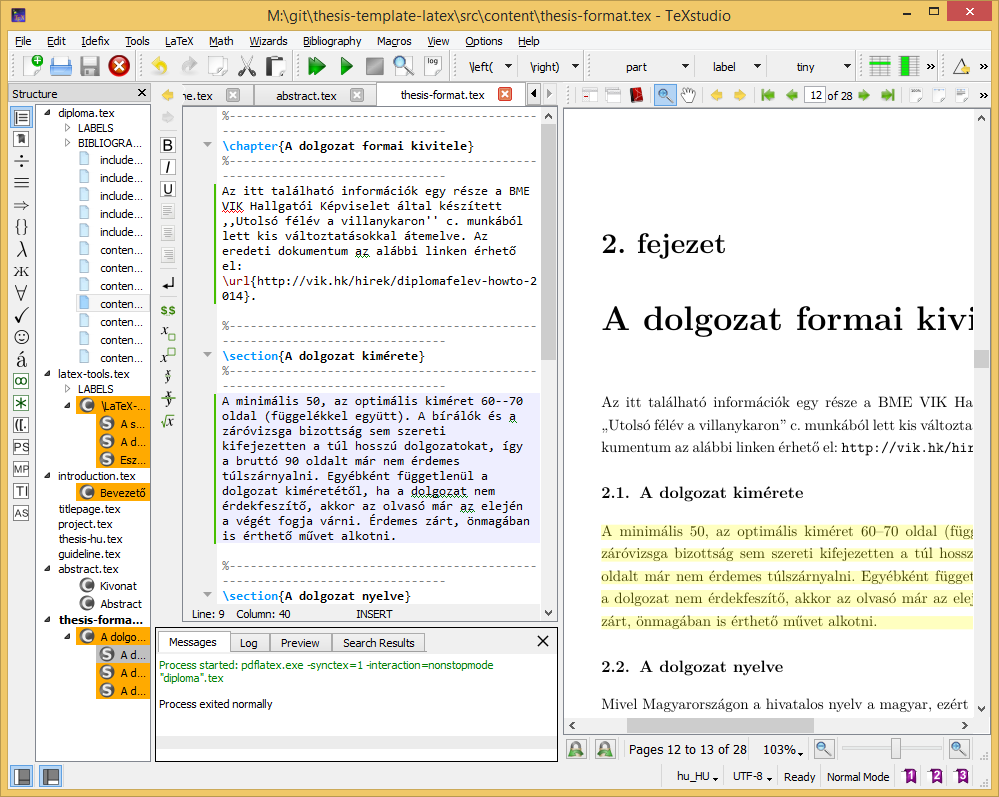
\includegraphics[width=150mm, keepaspectratio]{figures/TeXstudio.png}
\caption{A TeXstudio \LaTeX-szerkesztő.} 
\end{figure}

%----------------------------------------------------------------------------
\clearpage\section{Válasz az ,,Élet, a világmindenség, meg minden'' kérdésére}
%----------------------------------------------------------------------------
A Pitagorasz-tételből levezetve
\begin{align}
c^2=a^2+b^2=42.
\end{align}
A Faraday-indukciós törvényből levezetve
\begin{align}
\rot E=-\frac{dB}{dt}\hspace{1cm}\longrightarrow \hspace{1cm}
U_i=\oint\limits_\mathbf{L}{\mathbf{E}\mathbf{dl}}=-\frac{d}{dt}\int\limits_A{\mathbf{B}\mathbf{da}}=42.
\end{align}


%\label{page:last}
\end{document}
